% =====================================================================================
% Reproducing and Improving FiDIP for Infant Pose Estimation on SyRIP
% EECE 7373 Machine Learning with Small Data (Northeastern University), Fall 2026
%
% Build:  bash report/build.sh            (tectonic; writes report/FiDIP_Report.pdf)
% Overleaf: upload the report/ folder; set the compiler to pdfLaTeX (or XeLaTeX) and main
%           document to report.tex. Source is ASCII-only, so either engine works.
%
% Every experimental number is read from report/generated/*.tex (written by
% scripts/collect_results.py from eval/eval_coco.py outputs). Never type one by hand.
% Published baseline numbers are typed, always with a citation.
% =====================================================================================
\documentclass[11pt,letterpaper]{article}

\usepackage[margin=0.95in]{geometry}
\usepackage[T1]{fontenc}
\usepackage{lmodern}
\usepackage{microtype}
\usepackage{amsmath,amssymb}
\usepackage{graphicx}
\usepackage[table]{xcolor}
\usepackage{booktabs,array,multirow}
\usepackage{adjustbox}
\usepackage{enumitem}
\usepackage[font=small,labelfont=bf,skip=4pt]{caption}
\usepackage{subcaption}
\usepackage{tikz}
\usetikzlibrary{positioning,arrows.meta,fit,backgrounds,calc,shapes.geometric,decorations.pathreplacing,patterns}
\usepackage[most]{tcolorbox}
\usepackage{environ}
\usepackage{listings}
\usepackage[numbers,sort&compress]{natbib}
\PassOptionsToPackage{obeyspaces,spaces}{url}
\usepackage{xurl}
\usepackage[hidelinks]{hyperref}
\usepackage{doi}
\usepackage[capitalise,noabbrev]{cleveref}

\setlist{itemsep=1pt,topsep=3pt,parsep=0pt}
\setlength{\parskip}{2pt}
\setlength{\emergencystretch}{2em}
\urlstyle{same}
\DeclareUrlCommand\code{\urlstyle{tt}}   % \code{eval/eval_coco.py}: tt, breaks at / . _
\hypersetup{colorlinks=true, linkcolor=poseC!70!black, citecolor=poseC!70!black, urlcolor=poseC!70!black}

% ---- colours (Okabe-Ito based; colour-blind safe) -------------------------------------------
\definecolor{poseC}{HTML}{0072B2}   % pose network / our pipeline
\definecolor{domC}{HTML}{009E73}    % domain classifier / cluster
\definecolor{lossC}{HTML}{D55E00}   % losses / Test100
\definecolor{realC}{HTML}{E69F00}   % real images / human
\definecolor{synC}{HTML}{CC79A7}    % synthetic images
\definecolor{tbdred}{HTML}{C0392B}
\definecolor{interpbg}{gray}{0.93}

% ---- result store: \setres{key}{value} (generated) / \res{key} (prose and tables) -------------
\makeatletter
\newcounter{tbdcount}
\newcounter{interpcount}
\newcounter{pendingcount}
\newcommand{\tbd}{\stepcounter{tbdcount}\textcolor{tbdred}{\textbf{TBD}}}
\newcommand{\setres}[2]{\@namedef{res@#1}{#2}}
\newcommand{\setresdefault}[2]{\@ifundefined{res@#1}{\setres{#1}{#2}}{}}  % only if not set by a generated file
\newcommand{\setresmac}[2]{\setres{#1}{\@ifundefined{#2}{\textcolor{tbdred}{\textbf{??}}\PackageWarning{report}{Generated macro \string\#2\space missing (key #1)}}{\ensuremath{\@nameuse{#2}}}}}
\DeclareRobustCommand{\res}[1]{%
  \@ifundefined{res@#1}%
    {\textcolor{tbdred}{\textbf{??}}\PackageWarning{report}{Result key `#1' is not defined}}%
    {\@nameuse{res@#1}}}
\newcommand{\pm@sd}[2]{\res{#1}\,{\footnotesize$\pm$\,\res{#2}}}
\newcommand{\resms}[1]{\pm@sd{#1.mean}{#1.sd}}  % \resms{best.test.ap} -> mean +- sd
% ---- generated tables and figures (compile even before they exist) ----------------------------
\newcommand{\pendingbox}[1]{\stepcounter{pendingcount}\fbox{\parbox{0.9\linewidth}{\centering\small\color{tbdred}\textbf{Pending:} #1}}}
\newcommand{\GenTable}[2]{% #1 basename in generated/, #2 what it will contain
  \IfFileExists{generated/#1.tex}%
    {\begin{adjustbox}{max width=\linewidth}\input{generated/#1.tex}\end{adjustbox}}%
    {\pendingbox{\texttt{\detokenize{generated/#1.tex}} --- #2}}}
\newcommand{\figsearchdirs}{figures/generated/,../results/figures/,../results/figures/demo/}
\newcommand{\GenFigure}[3][width=\linewidth]{% #2 basename (no extension), #3 what it will show
  \gdef\gf@found{}%
  \@for\gf@dir:=\figsearchdirs\do{%
    \ifx\gf@found\@empty\IfFileExists{\gf@dir#2.pdf}{\xdef\gf@found{\gf@dir#2.pdf}}{}\fi
    \ifx\gf@found\@empty\IfFileExists{\gf@dir#2.png}{\xdef\gf@found{\gf@dir#2.png}}{}\fi
    \ifx\gf@found\@empty\IfFileExists{\gf@dir#2.jpg}{\xdef\gf@found{\gf@dir#2.jpg}}{}\fi}%
  \ifx\gf@found\@empty
    \pendingbox{figure \texttt{\detokenize{#2}}.\{pdf,png\} --- #3}%
  \else\includegraphics[#1]{\gf@found}\fi}
% ---- interpretation that can only be written once results exist --------------------------------
\newcommand{\interp}[1]{\stepcounter{interpcount}\par\smallskip\noindent
  \colorbox{interpbg}{\parbox{\dimexpr\linewidth-2\fboxsep\relax}{\small\itshape
  \textbf{Interpretation pending final results:} #1}}\par\smallskip}
\AtEndDocument{%
  \ifnum\value{tbdcount}>0 \PackageWarningNoLine{report}{\arabic{tbdcount} TBD placeholder value(s) typeset}\fi
  \ifnum\value{interpcount}>0 \PackageWarningNoLine{report}{\arabic{interpcount} interpretation placeholder(s) remain}\fi
  \ifnum\value{pendingcount}>0 \PackageWarningNoLine{report}{\arabic{pendingcount} pending generated file(s)}\fi}
\makeatother

% ---- misc -------------------------------------------------------------------------------------
\newcommand{\eg}{e.g.,\ }
\newcommand{\ie}{i.e.,\ }
\newcommand{\APstrict}{AP$_{80:95}$}
\newcommand{\lam}{\lambda}
\lstset{basicstyle=\ttfamily\footnotesize, columns=fullflexible, breaklines=true,
        frame=single, rulecolor=\color{black!25}, backgroundcolor=\color{black!3},
        xleftmargin=3pt, xrightmargin=3pt, aboveskip=4pt, belowskip=4pt, showstringspaces=false}
\newtcolorbox{keybox}[1]{enhanced, breakable, colback=poseC!4, colframe=poseC!75!black,
  fonttitle=\bfseries\sffamily, title={#1}, boxrule=0.7pt, arc=2pt, left=5pt, right=5pt, top=3pt, bottom=3pt}

% ---- generated values -------------------------------------------------------------------------
% 1. generated/results_tables.tex (scripts/collect_results.py): \newcommand macros, plus float tables.
%    Only its macros are taken here; its floats are discarded (the report places its own tables
%    from generated/tab_*.tex, so labels never clash).
\makeatletter
\IfFileExists{generated/results_tables.tex}{%
  \let\rt@table\table \let\rt@endtable\endtable
  \RenewEnviron{table}[1][]{}%
  % AUTO-GENERATED by scripts/collect_results.py -- do not edit by hand.
% Requires \usepackage{booktabs}. Numbers are percent (COCO keypoint AP x 100).
% Published numbers: github.com/ostadabbas/Infant-Pose-Estimation README @ a76b4f4 (Test100, GT boxes).

\newcommand{\PaperFiDIPAP}{93.6}  % github.com/ostadabbas/Infant-Pose-Estimation README @ a76b4f4 (Test100, GT boxes)
\newcommand{\PaperFiDIPAPFifty}{98.5}  % github.com/ostadabbas/Infant-Pose-Estimation README @ a76b4f4 (Test100, GT boxes)
\newcommand{\PaperFiDIPAPSeventyfive}{98.5}  % github.com/ostadabbas/Infant-Pose-Estimation README @ a76b4f4 (Test100, GT boxes)
\newcommand{\PaperFiDIPAR}{94.6}  % github.com/ostadabbas/Infant-Pose-Estimation README @ a76b4f4 (Test100, GT boxes)
\newcommand{\PaperFiDIPAPStrict}{86.25}  % implied: (10 AP - 6 AP50)/4, since AP50 = AP75 means AP is flat over .50-.75
\newcommand{\PaperFinetuneAP}{92.7}  % github.com/ostadabbas/Infant-Pose-Estimation README @ a76b4f4 (Test100, GT boxes)
\newcommand{\PaperFinetuneAPFifty}{98.5}  % github.com/ostadabbas/Infant-Pose-Estimation README @ a76b4f4 (Test100, GT boxes)
\newcommand{\PaperFinetuneAPSeventyfive}{98.5}  % github.com/ostadabbas/Infant-Pose-Estimation README @ a76b4f4 (Test100, GT boxes)
\newcommand{\PaperFinetuneAR}{93.9}  % github.com/ostadabbas/Infant-Pose-Estimation README @ a76b4f4 (Test100, GT boxes)
\newcommand{\PaperFinetuneAPStrict}{84.00}  % implied: (10 AP - 6 AP50)/4, since AP50 = AP75 means AP is flat over .50-.75
\newcommand{\PaperDarkPoseAP}{88.5}  % github.com/ostadabbas/Infant-Pose-Estimation README @ a76b4f4 (Test100, GT boxes)
\newcommand{\PaperDarkPoseAPFifty}{98.5}  % github.com/ostadabbas/Infant-Pose-Estimation README @ a76b4f4 (Test100, GT boxes)
\newcommand{\PaperDarkPoseAPSeventyfive}{98.5}  % github.com/ostadabbas/Infant-Pose-Estimation README @ a76b4f4 (Test100, GT boxes)
\newcommand{\PaperDarkPoseAR}{90.0}  % github.com/ostadabbas/Infant-Pose-Estimation README @ a76b4f4 (Test100, GT boxes)
\newcommand{\PaperDarkPoseAPStrict}{73.50}  % implied: (10 AP - 6 AP50)/4, since AP50 = AP75 means AP is flat over .50-.75
\newcommand{\RelFiDIPTestAP}{93.6}  % test100 paper: R001_fidip-w48_released
\newcommand{\RelFiDIPTestAPStrict}{86.2}  % test100 paper: R001_fidip-w48_released
\newcommand{\RelFiDIPTestAPFifty}{98.5}  % test100 paper: R001_fidip-w48_released
\newcommand{\RelFiDIPTestAPSeventyfive}{98.5}  % test100 paper: R001_fidip-w48_released
\newcommand{\RelFiDIPTestAR}{94.6}  % test100 paper: R001_fidip-w48_released
\newcommand{\RelFiDIPTestAPFixed}{95.0}  % test100 fixed: R001_fidip-w48_released
\newcommand{\RelFiDIPTestAPStrictFixed}{87.5}  % test100 fixed: R001_fidip-w48_released
\newcommand{\RelFiDIPValAP}{90.4}  % val400 paper: R001_fidip-w48_released
\newcommand{\RelFiDIPValAPStrict}{79.2}  % val400 paper: R001_fidip-w48_released
\newcommand{\RelFiDIPValAPFifty}{98.8}  % val400 paper: R001_fidip-w48_released
\newcommand{\RelFiDIPValAPSeventyfive}{95.8}  % val400 paper: R001_fidip-w48_released
\newcommand{\RelFiDIPValAR}{91.9}  % val400 paper: R001_fidip-w48_released
\newcommand{\RelFiDIPValAPFixed}{90.4}  % val400 fixed: R001_fidip-w48_released
\newcommand{\RelFiDIPValAPStrictFixed}{79.2}  % val400 fixed: R001_fidip-w48_released
\newcommand{\RelFiDIPTestCleanAP}{92.8}  % test100_clean paper: R001_fidip-w48_released
\newcommand{\RelFiDIPTestCleanAPStrict}{85.8}  % test100_clean paper: R001_fidip-w48_released
\newcommand{\RelFiDIPTestCleanAPFifty}{97.5}  % test100_clean paper: R001_fidip-w48_released
\newcommand{\RelFiDIPTestCleanAPSeventyfive}{97.5}  % test100_clean paper: R001_fidip-w48_released
\newcommand{\RelFiDIPTestCleanAR}{94.6}  % test100_clean paper: R001_fidip-w48_released
\newcommand{\RelFiDIPTestCleanAPFixed}{94.9}  % test100_clean fixed: R001_fidip-w48_released
\newcommand{\RelFiDIPTestCleanAPStrictFixed}{87.2}  % test100_clean fixed: R001_fidip-w48_released
\newcommand{\RelMobileTestAP}{79.1}  % test100 paper: R002_fidip-mobilenet_released
\newcommand{\RelMobileTestAPStrict}{54.7}  % test100 paper: R002_fidip-mobilenet_released
\newcommand{\RelMobileTestAPFifty}{99.0}  % test100 paper: R002_fidip-mobilenet_released
\newcommand{\RelMobileTestAPSeventyfive}{89.3}  % test100 paper: R002_fidip-mobilenet_released
\newcommand{\RelMobileTestAR}{84.1}  % test100 paper: R002_fidip-mobilenet_released
\newcommand{\RelMobileTestAPFixed}{79.8}  % test100 fixed: R002_fidip-mobilenet_released
\newcommand{\RelMobileTestAPStrictFixed}{55.0}  % test100 fixed: R002_fidip-mobilenet_released
\newcommand{\RelMobileValAP}{68.2}  % val400 paper: R002_fidip-mobilenet_released
\newcommand{\RelMobileValAPStrict}{38.0}  % val400 paper: R002_fidip-mobilenet_released
\newcommand{\RelMobileValAPFifty}{95.3}  % val400 paper: R002_fidip-mobilenet_released
\newcommand{\RelMobileValAPSeventyfive}{77.4}  % val400 paper: R002_fidip-mobilenet_released
\newcommand{\RelMobileValAR}{76.9}  % val400 paper: R002_fidip-mobilenet_released
\newcommand{\RelMobileValAPFixed}{68.2}  % val400 fixed: R002_fidip-mobilenet_released
\newcommand{\RelMobileValAPStrictFixed}{38.0}  % val400 fixed: R002_fidip-mobilenet_released
\newcommand{\RelMobileTestCleanAP}{77.9}  % test100_clean paper: R002_fidip-mobilenet_released
\newcommand{\RelMobileTestCleanAPStrict}{53.1}  % test100_clean paper: R002_fidip-mobilenet_released
\newcommand{\RelMobileTestCleanAPFifty}{98.0}  % test100_clean paper: R002_fidip-mobilenet_released
\newcommand{\RelMobileTestCleanAPSeventyfive}{88.1}  % test100_clean paper: R002_fidip-mobilenet_released
\newcommand{\RelMobileTestCleanAR}{83.6}  % test100_clean paper: R002_fidip-mobilenet_released
\newcommand{\RelMobileTestCleanAPFixed}{78.7}  % test100_clean fixed: R002_fidip-mobilenet_released
\newcommand{\RelMobileTestCleanAPStrictFixed}{53.5}  % test100_clean fixed: R002_fidip-mobilenet_released
\newcommand{\MmpHRNetValAP}{91.5}  % val400 paper: R101_mmp-hrnetw48_base_s1
\newcommand{\MmpHRNetValAPStrict}{81.6}  % val400 paper: R101_mmp-hrnetw48_base_s1
\newcommand{\MmpHRNetValAPFifty}{98.9}  % val400 paper: R101_mmp-hrnetw48_base_s1
\newcommand{\MmpHRNetValAPSeventyfive}{95.7}  % val400 paper: R101_mmp-hrnetw48_base_s1
\newcommand{\MmpHRNetValAR}{92.7}  % val400 paper: R101_mmp-hrnetw48_base_s1
\newcommand{\MmpHRNetValAPFixed}{91.5}  % val400 fixed: R101_mmp-hrnetw48_base_s1
\newcommand{\MmpHRNetValAPStrictFixed}{81.6}  % val400 fixed: R101_mmp-hrnetw48_base_s1
\newcommand{\MmpVitLTwoValAP}{92.8}  % val400 paper: R102_mmp-vitpose-l256_base_s1
\newcommand{\MmpVitLTwoValAPStrict}{84.8}  % val400 paper: R102_mmp-vitpose-l256_base_s1
\newcommand{\MmpVitLTwoValAPFifty}{98.8}  % val400 paper: R102_mmp-vitpose-l256_base_s1
\newcommand{\MmpVitLTwoValAPSeventyfive}{96.7}  % val400 paper: R102_mmp-vitpose-l256_base_s1
\newcommand{\MmpVitLTwoValAR}{94.1}  % val400 paper: R102_mmp-vitpose-l256_base_s1
\newcommand{\MmpVitLTwoValAPFixed}{92.8}  % val400 fixed: R102_mmp-vitpose-l256_base_s1
\newcommand{\MmpVitLTwoValAPStrictFixed}{84.8}  % val400 fixed: R102_mmp-vitpose-l256_base_s1
\newcommand{\MmpHRNetLrTwoValAP}{91.4}  % val400 paper: R106_mmp-hrnetw48_lr2e-4_s1
\newcommand{\MmpHRNetLrTwoValAPStrict}{81.9}  % val400 paper: R106_mmp-hrnetw48_lr2e-4_s1
\newcommand{\MmpHRNetLrTwoValAPFifty}{98.8}  % val400 paper: R106_mmp-hrnetw48_lr2e-4_s1
\newcommand{\MmpHRNetLrTwoValAPSeventyfive}{95.8}  % val400 paper: R106_mmp-hrnetw48_lr2e-4_s1
\newcommand{\MmpHRNetLrTwoValAR}{92.6}  % val400 paper: R106_mmp-hrnetw48_lr2e-4_s1
\newcommand{\MmpHRNetLrTwoValAPFixed}{91.4}  % val400 fixed: R106_mmp-hrnetw48_lr2e-4_s1
\newcommand{\MmpHRNetLrTwoValAPStrictFixed}{81.9}  % val400 fixed: R106_mmp-hrnetw48_lr2e-4_s1
\newcommand{\MmpVitLLrTwoValAP}{92.6}  % val400 paper: R108_mmp-vitpose-l256_lr2e-4_s1
\newcommand{\MmpVitLLrTwoValAPStrict}{84.7}  % val400 paper: R108_mmp-vitpose-l256_lr2e-4_s1
\newcommand{\MmpVitLLrTwoValAPFifty}{98.9}  % val400 paper: R108_mmp-vitpose-l256_lr2e-4_s1
\newcommand{\MmpVitLLrTwoValAPSeventyfive}{96.8}  % val400 paper: R108_mmp-vitpose-l256_lr2e-4_s1
\newcommand{\MmpVitLLrTwoValAR}{93.9}  % val400 paper: R108_mmp-vitpose-l256_lr2e-4_s1
\newcommand{\MmpVitLLrTwoValAPFixed}{92.6}  % val400 fixed: R108_mmp-vitpose-l256_lr2e-4_s1
\newcommand{\MmpVitLLrTwoValAPStrictFixed}{84.7}  % val400 fixed: R108_mmp-vitpose-l256_lr2e-4_s1
\newcommand{\ZsHRNetValAP}{86.5}  % val400 paper: R181_mmp-hrnetw48_zeroshot_s0
\newcommand{\ZsHRNetValAPStrict}{71.6}  % val400 paper: R181_mmp-hrnetw48_zeroshot_s0
\newcommand{\ZsHRNetValAPFifty}{98.9}  % val400 paper: R181_mmp-hrnetw48_zeroshot_s0
\newcommand{\ZsHRNetValAPSeventyfive}{92.8}  % val400 paper: R181_mmp-hrnetw48_zeroshot_s0
\newcommand{\ZsHRNetValAR}{88.3}  % val400 paper: R181_mmp-hrnetw48_zeroshot_s0
\newcommand{\ZsHRNetValAPFixed}{86.5}  % val400 fixed: R181_mmp-hrnetw48_zeroshot_s0
\newcommand{\ZsHRNetValAPStrictFixed}{71.6}  % val400 fixed: R181_mmp-hrnetw48_zeroshot_s0
\newcommand{\ZsVitLTwoValAP}{88.2}  % val400 paper: R182_mmp-vitpose-l256_zeroshot_s0
\newcommand{\ZsVitLTwoValAPStrict}{74.8}  % val400 paper: R182_mmp-vitpose-l256_zeroshot_s0
\newcommand{\ZsVitLTwoValAPFifty}{98.9}  % val400 paper: R182_mmp-vitpose-l256_zeroshot_s0
\newcommand{\ZsVitLTwoValAPSeventyfive}{94.8}  % val400 paper: R182_mmp-vitpose-l256_zeroshot_s0
\newcommand{\ZsVitLTwoValAR}{90.4}  % val400 paper: R182_mmp-vitpose-l256_zeroshot_s0
\newcommand{\ZsVitLTwoValAPFixed}{88.2}  % val400 fixed: R182_mmp-vitpose-l256_zeroshot_s0
\newcommand{\ZsVitLTwoValAPStrictFixed}{74.8}  % val400 fixed: R182_mmp-vitpose-l256_zeroshot_s0
\newcommand{\ZsVitLThreeValAP}{86.3}  % val400 paper: R183_mmp-vitpose-l384_zeroshot_s0
\newcommand{\ZsVitLThreeValAPStrict}{70.9}  % val400 paper: R183_mmp-vitpose-l384_zeroshot_s0
\newcommand{\ZsVitLThreeValAPFifty}{97.8}  % val400 paper: R183_mmp-vitpose-l384_zeroshot_s0
\newcommand{\ZsVitLThreeValAPSeventyfive}{93.7}  % val400 paper: R183_mmp-vitpose-l384_zeroshot_s0
\newcommand{\ZsVitLThreeValAR}{89.4}  % val400 paper: R183_mmp-vitpose-l384_zeroshot_s0
\newcommand{\ZsVitLThreeValAPFixed}{86.3}  % val400 fixed: R183_mmp-vitpose-l384_zeroshot_s0
\newcommand{\ZsVitLThreeValAPStrictFixed}{70.9}  % val400 fixed: R183_mmp-vitpose-l384_zeroshot_s0
\newcommand{\ZsVitHTwoValAP}{88.8}  % val400 paper: R184_mmp-vitpose-h256_zeroshot_s0
\newcommand{\ZsVitHTwoValAPStrict}{75.8}  % val400 paper: R184_mmp-vitpose-h256_zeroshot_s0
\newcommand{\ZsVitHTwoValAPFifty}{98.9}  % val400 paper: R184_mmp-vitpose-h256_zeroshot_s0
\newcommand{\ZsVitHTwoValAPSeventyfive}{94.6}  % val400 paper: R184_mmp-vitpose-h256_zeroshot_s0
\newcommand{\ZsVitHTwoValAR}{90.9}  % val400 paper: R184_mmp-vitpose-h256_zeroshot_s0
\newcommand{\ZsVitHTwoValAPFixed}{88.8}  % val400 fixed: R184_mmp-vitpose-h256_zeroshot_s0
\newcommand{\ZsVitHTwoValAPStrictFixed}{75.8}  % val400 fixed: R184_mmp-vitpose-h256_zeroshot_s0
\newcommand{\ZsVitHThreeValAP}{87.4}  % val400 paper: R185_mmp-vitpose-h384_zeroshot_s0
\newcommand{\ZsVitHThreeValAPStrict}{73.0}  % val400 paper: R185_mmp-vitpose-h384_zeroshot_s0
\newcommand{\ZsVitHThreeValAPFifty}{98.9}  % val400 paper: R185_mmp-vitpose-h384_zeroshot_s0
\newcommand{\ZsVitHThreeValAPSeventyfive}{94.5}  % val400 paper: R185_mmp-vitpose-h384_zeroshot_s0
\newcommand{\ZsVitHThreeValAR}{90.4}  % val400 paper: R185_mmp-vitpose-h384_zeroshot_s0
\newcommand{\ZsVitHThreeValAPFixed}{87.4}  % val400 fixed: R185_mmp-vitpose-h384_zeroshot_s0
\newcommand{\ZsVitHThreeValAPStrictFixed}{73.0}  % val400 fixed: R185_mmp-vitpose-h384_zeroshot_s0
\newcommand{\SmokeValAP}{90.3}  % val400 paper: R190_mmp-hrnetw48_smoke_s1,R191_mmp-vitpose-l384_smoke_s1
\newcommand{\SmokeValAPStrict}{79.2}  % val400 paper: R190_mmp-hrnetw48_smoke_s1,R191_mmp-vitpose-l384_smoke_s1
\newcommand{\SmokeValAPFifty}{98.9}  % val400 paper: R190_mmp-hrnetw48_smoke_s1,R191_mmp-vitpose-l384_smoke_s1
\newcommand{\SmokeValAPSeventyfive}{95.8}  % val400 paper: R190_mmp-hrnetw48_smoke_s1,R191_mmp-vitpose-l384_smoke_s1
\newcommand{\SmokeValAR}{92.0}  % val400 paper: R190_mmp-hrnetw48_smoke_s1,R191_mmp-vitpose-l384_smoke_s1
\newcommand{\SmokeValAPStd}{0.81}  % val400 paper: R190_mmp-hrnetw48_smoke_s1,R191_mmp-vitpose-l384_smoke_s1
\newcommand{\SmokeValNRuns}{2}  % val400 paper: R190_mmp-hrnetw48_smoke_s1,R191_mmp-vitpose-l384_smoke_s1
\newcommand{\SmokeValAPFixed}{90.3}  % val400 fixed: R190_mmp-hrnetw48_smoke_s1,R191_mmp-vitpose-l384_smoke_s1
\newcommand{\SmokeValAPStrictFixed}{79.2}  % val400 fixed: R190_mmp-hrnetw48_smoke_s1,R191_mmp-vitpose-l384_smoke_s1
\newcommand{\RtFiDIPTestAP}{93.6}  % test100 paper: R010_fidip-w48_lambda5e-4_s1,R011_fidip-w48_lambda5e-4_s2,R012_fidip-w48_lambda5e-4_s3
\newcommand{\RtFiDIPTestAPStrict}{86.2}  % test100 paper: R010_fidip-w48_lambda5e-4_s1,R011_fidip-w48_lambda5e-4_s2,R012_fidip-w48_lambda5e-4_s3
\newcommand{\RtFiDIPTestAPFifty}{98.5}  % test100 paper: R010_fidip-w48_lambda5e-4_s1,R011_fidip-w48_lambda5e-4_s2,R012_fidip-w48_lambda5e-4_s3
\newcommand{\RtFiDIPTestAPSeventyfive}{98.5}  % test100 paper: R010_fidip-w48_lambda5e-4_s1,R011_fidip-w48_lambda5e-4_s2,R012_fidip-w48_lambda5e-4_s3
\newcommand{\RtFiDIPTestAR}{94.6}  % test100 paper: R010_fidip-w48_lambda5e-4_s1,R011_fidip-w48_lambda5e-4_s2,R012_fidip-w48_lambda5e-4_s3
\newcommand{\RtFiDIPTestAPStd}{0.42}  % test100 paper: R010_fidip-w48_lambda5e-4_s1,R011_fidip-w48_lambda5e-4_s2,R012_fidip-w48_lambda5e-4_s3
\newcommand{\RtFiDIPTestNRuns}{3}  % test100 paper: R010_fidip-w48_lambda5e-4_s1,R011_fidip-w48_lambda5e-4_s2,R012_fidip-w48_lambda5e-4_s3
\newcommand{\RtFiDIPTestAPFixed}{95.1}  % test100 fixed: R010_fidip-w48_lambda5e-4_s1,R011_fidip-w48_lambda5e-4_s2,R012_fidip-w48_lambda5e-4_s3
\newcommand{\RtFiDIPTestAPStrictFixed}{87.8}  % test100 fixed: R010_fidip-w48_lambda5e-4_s1,R011_fidip-w48_lambda5e-4_s2,R012_fidip-w48_lambda5e-4_s3
\newcommand{\RtFiDIPValAP}{90.5}  % val400 paper: R010_fidip-w48_lambda5e-4_s1,R011_fidip-w48_lambda5e-4_s2,R012_fidip-w48_lambda5e-4_s3
\newcommand{\RtFiDIPValAPStrict}{79.6}  % val400 paper: R010_fidip-w48_lambda5e-4_s1,R011_fidip-w48_lambda5e-4_s2,R012_fidip-w48_lambda5e-4_s3
\newcommand{\RtFiDIPValAPFifty}{98.8}  % val400 paper: R010_fidip-w48_lambda5e-4_s1,R011_fidip-w48_lambda5e-4_s2,R012_fidip-w48_lambda5e-4_s3
\newcommand{\RtFiDIPValAPSeventyfive}{95.8}  % val400 paper: R010_fidip-w48_lambda5e-4_s1,R011_fidip-w48_lambda5e-4_s2,R012_fidip-w48_lambda5e-4_s3
\newcommand{\RtFiDIPValAR}{91.9}  % val400 paper: R010_fidip-w48_lambda5e-4_s1,R011_fidip-w48_lambda5e-4_s2,R012_fidip-w48_lambda5e-4_s3
\newcommand{\RtFiDIPValAPStd}{0.13}  % val400 paper: R010_fidip-w48_lambda5e-4_s1,R011_fidip-w48_lambda5e-4_s2,R012_fidip-w48_lambda5e-4_s3
\newcommand{\RtFiDIPValNRuns}{3}  % val400 paper: R010_fidip-w48_lambda5e-4_s1,R011_fidip-w48_lambda5e-4_s2,R012_fidip-w48_lambda5e-4_s3
\newcommand{\RtFiDIPValAPFixed}{90.5}  % val400 fixed: R010_fidip-w48_lambda5e-4_s1,R011_fidip-w48_lambda5e-4_s2,R012_fidip-w48_lambda5e-4_s3
\newcommand{\RtFiDIPValAPStrictFixed}{79.6}  % val400 fixed: R010_fidip-w48_lambda5e-4_s1,R011_fidip-w48_lambda5e-4_s2,R012_fidip-w48_lambda5e-4_s3
\newcommand{\RtFiDIPTestCleanAP}{92.8}  % test100_clean paper: R010_fidip-w48_lambda5e-4_s1,R011_fidip-w48_lambda5e-4_s2,R012_fidip-w48_lambda5e-4_s3
\newcommand{\RtFiDIPTestCleanAPStrict}{85.9}  % test100_clean paper: R010_fidip-w48_lambda5e-4_s1,R011_fidip-w48_lambda5e-4_s2,R012_fidip-w48_lambda5e-4_s3
\newcommand{\RtFiDIPTestCleanAPFifty}{97.5}  % test100_clean paper: R010_fidip-w48_lambda5e-4_s1,R011_fidip-w48_lambda5e-4_s2,R012_fidip-w48_lambda5e-4_s3
\newcommand{\RtFiDIPTestCleanAPSeventyfive}{97.5}  % test100_clean paper: R010_fidip-w48_lambda5e-4_s1,R011_fidip-w48_lambda5e-4_s2,R012_fidip-w48_lambda5e-4_s3
\newcommand{\RtFiDIPTestCleanAR}{94.7}  % test100_clean paper: R010_fidip-w48_lambda5e-4_s1,R011_fidip-w48_lambda5e-4_s2,R012_fidip-w48_lambda5e-4_s3
\newcommand{\RtFiDIPTestCleanAPStd}{0.40}  % test100_clean paper: R010_fidip-w48_lambda5e-4_s1,R011_fidip-w48_lambda5e-4_s2,R012_fidip-w48_lambda5e-4_s3
\newcommand{\RtFiDIPTestCleanNRuns}{3}  % test100_clean paper: R010_fidip-w48_lambda5e-4_s1,R011_fidip-w48_lambda5e-4_s2,R012_fidip-w48_lambda5e-4_s3
\newcommand{\RtFiDIPTestCleanAPFixed}{95.0}  % test100_clean fixed: R010_fidip-w48_lambda5e-4_s1,R011_fidip-w48_lambda5e-4_s2,R012_fidip-w48_lambda5e-4_s3
\newcommand{\RtFiDIPTestCleanAPStrictFixed}{87.4}  % test100_clean fixed: R010_fidip-w48_lambda5e-4_s1,R011_fidip-w48_lambda5e-4_s2,R012_fidip-w48_lambda5e-4_s3
\newcommand{\MmpVitLLrFiveValAP}{92.6}  % val400 paper: R109_mmp-vitpose-l256_lr5e-5_s1
\newcommand{\MmpVitLLrFiveValAPStrict}{84.3}  % val400 paper: R109_mmp-vitpose-l256_lr5e-5_s1
\newcommand{\MmpVitLLrFiveValAPFifty}{98.8}  % val400 paper: R109_mmp-vitpose-l256_lr5e-5_s1
\newcommand{\MmpVitLLrFiveValAPSeventyfive}{96.7}  % val400 paper: R109_mmp-vitpose-l256_lr5e-5_s1
\newcommand{\MmpVitLLrFiveValAR}{94.0}  % val400 paper: R109_mmp-vitpose-l256_lr5e-5_s1
\newcommand{\MmpVitLLrFiveValAPFixed}{92.6}  % val400 fixed: R109_mmp-vitpose-l256_lr5e-5_s1
\newcommand{\MmpVitLLrFiveValAPStrictFixed}{84.3}  % val400 fixed: R109_mmp-vitpose-l256_lr5e-5_s1
\newcommand{\MmpVitHTwoValAP}{93.2}  % val400 paper: R105_mmp-vitpose-h256_base_s1
\newcommand{\MmpVitHTwoValAPStrict}{85.3}  % val400 paper: R105_mmp-vitpose-h256_base_s1
\newcommand{\MmpVitHTwoValAPFifty}{98.8}  % val400 paper: R105_mmp-vitpose-h256_base_s1
\newcommand{\MmpVitHTwoValAPSeventyfive}{97.6}  % val400 paper: R105_mmp-vitpose-h256_base_s1
\newcommand{\MmpVitHTwoValAR}{94.5}  % val400 paper: R105_mmp-vitpose-h256_base_s1
\newcommand{\MmpVitHTwoValAPFixed}{93.2}  % val400 fixed: R105_mmp-vitpose-h256_base_s1
\newcommand{\MmpVitHTwoValAPStrictFixed}{85.3}  % val400 fixed: R105_mmp-vitpose-h256_base_s1
\newcommand{\MmpVitHThreeValAP}{93.3}  % val400 paper: R104_mmp-vitpose-h384_base_s1
\newcommand{\MmpVitHThreeValAPStrict}{85.8}  % val400 paper: R104_mmp-vitpose-h384_base_s1
\newcommand{\MmpVitHThreeValAPFifty}{98.9}  % val400 paper: R104_mmp-vitpose-h384_base_s1
\newcommand{\MmpVitHThreeValAPSeventyfive}{96.7}  % val400 paper: R104_mmp-vitpose-h384_base_s1
\newcommand{\MmpVitHThreeValAR}{94.7}  % val400 paper: R104_mmp-vitpose-h384_base_s1
\newcommand{\MmpVitHThreeValAPFixed}{93.3}  % val400 fixed: R104_mmp-vitpose-h384_base_s1
\newcommand{\MmpVitHThreeValAPStrictFixed}{85.8}  % val400 fixed: R104_mmp-vitpose-h384_base_s1
\newcommand{\ReproSmokeValAP}{88.1}  % val400 paper: R009_fidip-w48_smoke_s1
\newcommand{\ReproSmokeValAPStrict}{74.7}  % val400 paper: R009_fidip-w48_smoke_s1
\newcommand{\ReproSmokeValAPFifty}{98.9}  % val400 paper: R009_fidip-w48_smoke_s1
\newcommand{\ReproSmokeValAPSeventyfive}{93.8}  % val400 paper: R009_fidip-w48_smoke_s1
\newcommand{\ReproSmokeValAR}{89.8}  % val400 paper: R009_fidip-w48_smoke_s1
\newcommand{\ReproSmokeValAPFixed}{88.1}  % val400 fixed: R009_fidip-w48_smoke_s1
\newcommand{\ReproSmokeValAPStrictFixed}{74.7}  % val400 fixed: R009_fidip-w48_smoke_s1
\newcommand{\RtLamOneEFourValAP}{91.0}  % val400 paper: R016_fidip-w48_lambda1e-4_s1
\newcommand{\RtLamOneEFourValAPStrict}{80.3}  % val400 paper: R016_fidip-w48_lambda1e-4_s1
\newcommand{\RtLamOneEFourValAPFifty}{98.8}  % val400 paper: R016_fidip-w48_lambda1e-4_s1
\newcommand{\RtLamOneEFourValAPSeventyfive}{96.8}  % val400 paper: R016_fidip-w48_lambda1e-4_s1
\newcommand{\RtLamOneEFourValAR}{92.3}  % val400 paper: R016_fidip-w48_lambda1e-4_s1
\newcommand{\RtLamOneEFourValAPFixed}{91.0}  % val400 fixed: R016_fidip-w48_lambda1e-4_s1
\newcommand{\RtLamOneEFourValAPStrictFixed}{80.3}  % val400 fixed: R016_fidip-w48_lambda1e-4_s1
\newcommand{\RtLamTwoEThreeValAP}{89.7}  % val400 paper: R017_fidip-w48_lambda2e-3_s1
\newcommand{\RtLamTwoEThreeValAPStrict}{77.8}  % val400 paper: R017_fidip-w48_lambda2e-3_s1
\newcommand{\RtLamTwoEThreeValAPFifty}{98.9}  % val400 paper: R017_fidip-w48_lambda2e-3_s1
\newcommand{\RtLamTwoEThreeValAPSeventyfive}{95.8}  % val400 paper: R017_fidip-w48_lambda2e-3_s1
\newcommand{\RtLamTwoEThreeValAR}{91.2}  % val400 paper: R017_fidip-w48_lambda2e-3_s1
\newcommand{\RtLamTwoEThreeValAPFixed}{89.7}  % val400 fixed: R017_fidip-w48_lambda2e-3_s1
\newcommand{\RtLamTwoEThreeValAPStrictFixed}{77.8}  % val400 fixed: R017_fidip-w48_lambda2e-3_s1
\newcommand{\RtLamOneETwoValAP}{85.8}  % val400 paper: R018_fidip-w48_lambda1e-2_s1
\newcommand{\RtLamOneETwoValAPStrict}{70.0}  % val400 paper: R018_fidip-w48_lambda1e-2_s1
\newcommand{\RtLamOneETwoValAPFifty}{98.9}  % val400 paper: R018_fidip-w48_lambda1e-2_s1
\newcommand{\RtLamOneETwoValAPSeventyfive}{92.7}  % val400 paper: R018_fidip-w48_lambda1e-2_s1
\newcommand{\RtLamOneETwoValAR}{87.8}  % val400 paper: R018_fidip-w48_lambda1e-2_s1
\newcommand{\RtLamOneETwoValAPFixed}{85.8}  % val400 fixed: R018_fidip-w48_lambda1e-2_s1
\newcommand{\RtLamOneETwoValAPStrictFixed}{70.0}  % val400 fixed: R018_fidip-w48_lambda1e-2_s1
\newcommand{\MmpVitLThreeValAP}{92.8}  % val400 paper: R103_mmp-vitpose-l384_base_s1
\newcommand{\MmpVitLThreeValAPStrict}{84.8}  % val400 paper: R103_mmp-vitpose-l384_base_s1
\newcommand{\MmpVitLThreeValAPFifty}{98.8}  % val400 paper: R103_mmp-vitpose-l384_base_s1
\newcommand{\MmpVitLThreeValAPSeventyfive}{96.6}  % val400 paper: R103_mmp-vitpose-l384_base_s1
\newcommand{\MmpVitLThreeValAR}{94.2}  % val400 paper: R103_mmp-vitpose-l384_base_s1
\newcommand{\MmpVitLThreeValAPFixed}{92.8}  % val400 fixed: R103_mmp-vitpose-l384_base_s1
\newcommand{\MmpVitLThreeValAPStrictFixed}{84.8}  % val400 fixed: R103_mmp-vitpose-l384_base_s1
\newcommand{\MmpHRNetLrFiveValAP}{91.7}  % val400 paper: R107_mmp-hrnetw48_lr5e-5_s1
\newcommand{\MmpHRNetLrFiveValAPStrict}{81.7}  % val400 paper: R107_mmp-hrnetw48_lr5e-5_s1
\newcommand{\MmpHRNetLrFiveValAPFifty}{98.9}  % val400 paper: R107_mmp-hrnetw48_lr5e-5_s1
\newcommand{\MmpHRNetLrFiveValAPSeventyfive}{96.7}  % val400 paper: R107_mmp-hrnetw48_lr5e-5_s1
\newcommand{\MmpHRNetLrFiveValAR}{92.8}  % val400 paper: R107_mmp-hrnetw48_lr5e-5_s1
\newcommand{\MmpHRNetLrFiveValAPFixed}{91.7}  % val400 fixed: R107_mmp-hrnetw48_lr5e-5_s1
\newcommand{\MmpHRNetLrFiveValAPStrictFixed}{81.7}  % val400 fixed: R107_mmp-hrnetw48_lr5e-5_s1
\newcommand{\MmpVitLRealValAP}{92.2}  % val400 paper: R120_mmp-vitpose-l256_realonly_s1
\newcommand{\MmpVitLRealValAPStrict}{83.4}  % val400 paper: R120_mmp-vitpose-l256_realonly_s1
\newcommand{\MmpVitLRealValAPFifty}{98.8}  % val400 paper: R120_mmp-vitpose-l256_realonly_s1
\newcommand{\MmpVitLRealValAPSeventyfive}{96.8}  % val400 paper: R120_mmp-vitpose-l256_realonly_s1
\newcommand{\MmpVitLRealValAR}{93.8}  % val400 paper: R120_mmp-vitpose-l256_realonly_s1
\newcommand{\MmpVitLRealValAPFixed}{92.2}  % val400 fixed: R120_mmp-vitpose-l256_realonly_s1
\newcommand{\MmpVitLRealValAPStrictFixed}{83.4}  % val400 fixed: R120_mmp-vitpose-l256_realonly_s1
\newcommand{\MmpVitLRotValAP}{92.6}  % val400 paper: R121_mmp-vitpose-l256_rot180_s1
\newcommand{\MmpVitLRotValAPStrict}{84.3}  % val400 paper: R121_mmp-vitpose-l256_rot180_s1
\newcommand{\MmpVitLRotValAPFifty}{98.8}  % val400 paper: R121_mmp-vitpose-l256_rot180_s1
\newcommand{\MmpVitLRotValAPSeventyfive}{96.7}  % val400 paper: R121_mmp-vitpose-l256_rot180_s1
\newcommand{\MmpVitLRotValAR}{94.0}  % val400 paper: R121_mmp-vitpose-l256_rot180_s1
\newcommand{\MmpVitLRotValAPFixed}{92.6}  % val400 fixed: R121_mmp-vitpose-l256_rot180_s1
\newcommand{\MmpVitLRotValAPStrictFixed}{84.3}  % val400 fixed: R121_mmp-vitpose-l256_rot180_s1
\newcommand{\RelFiDIPTestAPCiLo}{89.8}  % test100 bootstrap: R001_fidip-w48_released
\newcommand{\RelFiDIPTestAPCiHi}{96.3}  % test100 bootstrap: R001_fidip-w48_released
\newcommand{\RelFiDIPValAPCiLo}{88.7}  % val400 bootstrap: R001_fidip-w48_released
\newcommand{\RelFiDIPValAPCiHi}{92.1}  % val400 bootstrap: R001_fidip-w48_released
\newcommand{\RelMobileTestAPCiLo}{74.3}  % test100 bootstrap: R002_fidip-mobilenet_released
\newcommand{\RelMobileTestAPCiHi}{83.8}  % test100 bootstrap: R002_fidip-mobilenet_released
\newcommand{\RelMobileValAPCiLo}{65.1}  % val400 bootstrap: R002_fidip-mobilenet_released
\newcommand{\RelMobileValAPCiHi}{71.6}  % val400 bootstrap: R002_fidip-mobilenet_released

\begin{table}[t]
\centering
\small
\caption{Reproduction on SyRIP Test100 (GT boxes). Paper protocol unless marked; ``fixed'' removes the pycocotools annotation-id-0 artefact (Sec.~\ref{sec:eval}). Mean\,$\pm$\,std over seeds. AP$_{.80:.95}$ for the paper rows is implied by AP, AP$_{50}$ and AP$_{75}$. Val400 is the selection split.}
\label{tab:repro}
\begin{tabular}{lrrrrrrrr}
\toprule
Model & runs & AP & AP$_{50}$ & AP$_{75}$ & AR & AP$_{.80:.95}$ & AP (fixed) & Val400 AP \\
\midrule
DarkPose + FiDIP (paper) & -- & 93.6 & 98.5 & 98.5 & 94.6 & 86.25 & -- & -- \\
DarkPose + Finetune (paper) & -- & 92.7 & 98.5 & 98.5 & 93.9 & 84.00 & -- & -- \\
DarkPose, no fine-tuning (paper) & -- & 88.5 & 98.5 & 98.5 & 90.0 & 73.50 & -- & -- \\
FiDIP HRNet-W48 (released) & 1 & 93.6 & 98.5 & 98.5 & 94.6 & 86.2 & 95.0 & 90.4 \\
FiDIP MobileNetV2 (released) & 1 & 79.1 & 99.0 & 89.3 & 84.1 & 54.7 & 79.8 & 68.2 \\
FiDIP retrain, \$\textbackslash{}lambda=5\textbackslash{}cdot10^{-4}\$ & 3 & 93.6\,$\pm$\,0.4 & 98.5 & 98.5 & 94.6 & 86.2 & 95.1 & 90.5\,$\pm$\,0.1 \\
Fine-tune retrain, \$\textbackslash{}lambda=0\$ & -- & -- & -- & -- & -- & -- & -- & -- \\
\bottomrule
\end{tabular}
\end{table}

\begin{table}[t]
\centering
\small
\caption{Main comparison on the clean Test100 split. Only released/retrained reproduction targets and pre-registered configurations are evaluated on Test100.}
\label{tab:main}
\begin{tabular}{lrrrrrrrr}
\toprule
Model & runs & AP & AP$_{50}$ & AP$_{75}$ & AR & AP$_{.80:.95}$ & AP (fixed) & Val400 AP \\
\midrule
DarkPose + FiDIP (paper) & -- & 93.6 & 98.5 & 98.5 & 94.6 & 86.25 & -- & -- \\
FiDIP HRNet-W48 (released) & 1 & 93.6 & 98.5 & 98.5 & 94.6 & 86.2 & 95.0 & 90.4 \\
FiDIP MobileNetV2 (released) & 1 & 79.1 & 99.0 & 89.3 & 84.1 & 54.7 & 79.8 & 68.2 \\
FiDIP retrain, \$\textbackslash{}lambda=5\textbackslash{}cdot10^{-4}\$ & 3 & 93.6\,$\pm$\,0.4 & 98.5 & 98.5 & 94.6 & 86.2 & 95.1 & 90.5 \\
\bottomrule
\end{tabular}
\end{table}

\begin{table}[t]
\centering
\small
\caption{Every attempt and its accuracy. Val400 AP drives every decision. Test100 is shown only for reproduction targets and pre-registered finalists (``withheld'' otherwise). Smoke runs (pipeline checks) are listed in results/tables/attempts.csv only.}
\label{tab:attempts}
\begin{tabular}{rllrrr}
\toprule
\# & Configuration & What changed & runs & Val400 AP & Test100 AP \\
\midrule
1 & FiDIP HRNet-W48 (released) & upstream hrnet\_fidip.pth, upstream test code & 1 & 90.4 & 93.6 \\
2 & FiDIP MobileNetV2 (released) & upstream mobile\_fidip.pth, 224x224 & 1 & 68.2 & 79.1 \\
3 & HRNet-W48 DARK 384 (MMPose control) & FiDIP backbone re-implemented in MMPose, no domain adaptation, shared recipe & 1 & 91.5 & withheld \\
4 & ViTPose-L 256 (MMPose) & backbone HRNet-W48 -> ViTPose-L (UDP, 256x192), same recipe & 1 & 92.8 & withheld \\
5 & HRNet-W48 DARK 384, LR 2e-4 & control with LR 1e-4 -> 2e-4 & 1 & 91.4 & withheld \\
6 & ViTPose-L 256, LR 2e-4 & ViTPose-L 256 with LR 1e-4 -> 2e-4 & 1 & 92.6 & withheld \\
7 & HRNet-W48 COCO, zero-shot & no infant training (MMPose COCO checkpoint) & 1 & 86.5 & withheld \\
8 & ViTPose-L 256 COCO, zero-shot & no infant training & 1 & 88.2 & withheld \\
9 & ViTPose-L 384 COCO, zero-shot & no infant training (pos-embed resized to 24x18) & 1 & 86.3 & withheld \\
10 & ViTPose-H 256 COCO, zero-shot & no infant training & 1 & 88.8 & withheld \\
11 & ViTPose-H 384 COCO, zero-shot & no infant training (pos-embed resized to 24x18) & 1 & 87.4 & withheld \\
13 & FiDIP retrain, \$\textbackslash{}lambda=5\textbackslash{}cdot10^{-4}\$ & official recipe retrain (COCO DarkPose init, PRE\_EPOCH 10, lambda 5e-4), Val400 epoch selection & 3 & 90.5\,$\pm$\,0.1 & 93.6\,$\pm$\,0.4 \\
14 & Fine-tune retrain, \$\textbackslash{}lambda=0\$ & same recipe with lambda = 0 (no domain adaptation) & 3 & -- & withheld \\
15 & ViTPose-L 256, LR 5e-5 & ViTPose-L 256 with LR 1e-4 -> 5e-5 & 1 & 92.6 & withheld \\
16 & ViTPose-H 256 (MMPose) & backbone -> ViTPose-H (UDP, 256x192), same recipe & 1 & 93.2 & withheld \\
17 & ViTPose-H 384 (MMPose) & backbone -> ViTPose-H (UDP, 384x288), same recipe & 1 & 93.3 & withheld \\
19 & FiDIP retrain, lambda 1e-4 & domain-adaptation weight lambda 5e-4 -> 1e-4 (1 seed) & 1 & 91.0 & withheld \\
20 & FiDIP retrain, lambda 2e-3 & domain-adaptation weight lambda 5e-4 -> 2e-3 (1 seed) & 1 & 89.7 & withheld \\
21 & FiDIP retrain, lambda 1e-2 & domain-adaptation weight lambda 5e-4 -> 1e-2 (1 seed) & 1 & 85.8 & withheld \\
22 & ViTPose-L 384 (MMPose) & backbone -> ViTPose-L (UDP, 384x288), same recipe & 1 & 92.8 & withheld \\
23 & HRNet-W48 DARK 384, LR 5e-5 & control with LR 1e-4 -> 5e-5 & 1 & 91.7 & withheld \\
24 & ViTPose-L 256, real only & train on the 200 real images only (no synthetic) & 1 & 92.2 & withheld \\
25 & ViTPose-L 256, rotation \$\textbackslash{}pm\$180 & rotation augmentation up to 180 degrees & 1 & 92.6 & withheld \\
26 & Fine-tune retrain, attempt 1 & lambda = 0 retrain, first submission & 1 & -- & withheld \\
27 & HRNet-W48 DARK 384 (MMPose control) [noflip] & test-time: noflip & 1 & 90.9 & withheld \\
28 & ViTPose-L 256 (MMPose) [noflip] & test-time: noflip & 1 & 92.3 & withheld \\
\bottomrule
\end{tabular}
\end{table}

%
  \let\table\rt@table \let\endtable\rt@endtable}{}
\makeatother
% 2. generated/numbers.tex: the report's canonical keys, \setres{<key>}{<value or generated macro>}.
% 3. keymap.tex (optional, hand-maintained, no numbers): \setres{<key>}{\SomeGeneratedMacro}.
\IfFileExists{generated/numbers.tex}{% =====================================================================================
% report/generated/numbers.tex  --  PLACEHOLDER. Overwritten by scripts/collect_results.py.
% =====================================================================================
% Interface (owned by the report stream; filled by the analysis stream):
%   * One line per scalar:   \setres{<key>}{<value>}
%   * Keys are plain strings (dots/digits allowed). The report reads them with \res{<key>}.
%   * Any key that is never set prints a red "??" in the PDF and a LaTeX warning naming it,
%     so a partial file still compiles. Values left as \tbd print a red "TBD".
%   * Value formats:
%       AP-type metrics ........ percent, one decimal, no % sign:      93.6
%       std / CI bounds ........ percent, one decimal:                 0.4
%       signed differences ..... math-mode sign:                       $+0.8$   $-0.3$
%       p-values ............... 3 decimals or a bound:                0.012    $<$0.001
%       names .................. LaTeX-safe text:                      ViTPose-H 384$\times$288
%       commit SHAs ............ \texttt{} short SHA:                  \texttt{1a2b3c4}
%   * A value may also be a macro from generated/results_tables.tex, e.g. \setres{rel.fidip.test.ap}{\RelFiDIPTestAP};
%     report/keymap.tex (loaded after this file) can hold such mappings by hand -- it never holds numbers.
%   * Every number must come from eval/eval_coco.py / eval/bootstrap_ci.py outputs (CLAUDE.md).
%     Protocol = `paper` (annotation ids as shipped) unless the key says `.fixed`.
% =====================================================================================

% ---- Released checkpoints, evaluated by eval/eval_coco.py (reproduction targets) ----------
\setres{rel.fidip.test.ap}{\tbd}          % R001 hrnet_fidip.pth, Test100 AP (paper protocol)
\setres{rel.fidip.test.ap50}{\tbd}        % ... AP50
\setres{rel.fidip.test.ap75}{\tbd}        % ... AP75
\setres{rel.fidip.test.ar}{\tbd}          % ... AR
\setres{rel.fidip.test.apstrict}{\tbd}    % ... AP_80_95 (mean AP over OKS 0.80..0.95)
\setres{rel.fidip.test.ap.fixed}{\tbd}    % ... Test100 AP, `fixed` protocol (ids shifted off 0)
\setres{rel.fidip.test.ar.fixed}{\tbd}    % ... AR, `fixed` protocol
\setres{rel.fidip.test.diffpub}{\tbd}     % rel.fidip.test.ap - 93.6, signed
\setres{rel.fidip.test.ap.upstream}{\tbd} % AP printed by upstream tools/test_adaptive_model.py (cross-check)
\setres{rel.fidip.val.ap}{\tbd}           % R001 Val400 AP
\setres{rel.fidip.test.clean.ap}{\tbd}    % R001 AP on Test100-clean (95 images: Test100 minus the 5 copies of training images, D16)
\setres{rel.fidip.test0rank}{\tbd}       % R001: rank of test0's score among the 100 Test100 detections (D13)
\setres{rel.mobile.test.ap}{\tbd}         % R002 mobile_fidip.pth, Test100 AP (published: 79.2)
\setres{rel.mobile.val.ap}{\tbd}          % R002 Val400 AP
\setres{zs.darkpose.test.ap}{\tbd}        % COCO DarkPose W48 384x288, no infant training, Test100 AP (published: 88.5)
\setres{zs.darkpose.val.ap}{\tbd}         % ... Val400 AP

% ---- Retraining with the released recipe (+ TRAIN.CHECKPOINT = COCO DarkPose), Val400 selection
\setres{rt.seeds}{\tbd}                   % number of seeds per arm (e.g. 3)
\setres{rt.epochs}{\tbd}                  % epoch budget of the retrain (yaml: 20)
\setres{rt.fidip.test.ap.mean}{\tbd}      % FiDIP (lambda = 5e-4): Test100 AP, mean over seeds
\setres{rt.fidip.test.ap.sd}{\tbd}        % ... sample std over seeds
\setres{rt.fidip.val.ap.mean}{\tbd}       % ... Val400 AP mean
\setres{rt.fidip.val.ap.sd}{\tbd}         % ... Val400 AP std
\setres{rt.ft.test.ap.mean}{\tbd}         % plain fine-tune (lambda = 0): Test100 AP mean
\setres{rt.ft.test.ap.sd}{\tbd}
\setres{rt.ft.val.ap.mean}{\tbd}
\setres{rt.ft.val.ap.sd}{\tbd}
\setres{rt.delta.test.ap}{\tbd}           % FiDIP - fine-tune, seed-averaged Test100 AP, signed
\setres{rt.delta.test.ci.lo}{\tbd}        % 95% CI (bootstrap_ci.py multiseed), signed
\setres{rt.delta.test.ci.hi}{\tbd}
\setres{rt.delta.test.p}{\tbd}            % one-sided p (H1: FiDIP > fine-tune)
\setres{rt.fidip.bestepoch}{\tbd}         % median Val400-selected epoch, FiDIP arm (e.g. "14 of 20")
\setres{rt.ft.bestepoch}{\tbd}            % same, fine-tune arm

% ---- Improvement study (MMPose; all selection on Val400) ------------------------------------
\setres{imp.control.name}{\tbd}           % control, e.g. HRNet-W48 DARK 384$\times$288 (MMPose)
\setres{imp.control.val.ap.mean}{\tbd}    % control Val400 AP mean over seeds
\setres{imp.control.val.ap.sd}{\tbd}
\setres{best.name}{\tbd}                  % final pre-registered configuration, short name
\setres{best.input}{\tbd}                 % input size, e.g. 384$\times$288
\setres{best.flip}{\tbd}                  % flip test at inference: yes / no
\setres{best.ckptrule}{\tbd}              % checkpoint rule, e.g. "best Val400 AP epoch"
\setres{best.seeds}{\tbd}                 % number of seeds evaluated on Test100
\setres{best.prereg.commit}{\tbd}         % commit that registered it in results/PREREGISTRATION.md
\setres{best.val.ap.mean}{\tbd}           % Val400 AP mean over seeds
\setres{best.val.ap.sd}{\tbd}
\setres{best.test.ap.mean}{\tbd}          % Test100 AP mean over seeds (paper protocol)  <- headline
\setres{best.test.ap.sd}{\tbd}
\setres{best.test.ap50}{\tbd}             % seed means
\setres{best.test.ap75}{\tbd}
\setres{best.test.ar}{\tbd}
\setres{best.test.apstrict}{\tbd}         % AP_80_95, seed mean
\setres{best.test.ap.fixed}{\tbd}         % Test100 AP mean, `fixed` protocol
\setres{best.vs.published}{\tbd}          % best.test.ap.mean - 93.6, signed
\setres{best.delta.ap}{\tbd}              % vs released FiDIP (R001) on the same 100 images, signed
\setres{best.delta.ci.lo}{\tbd}           % 95% paired image-bootstrap CI (seed-averaged), signed
\setres{best.delta.ci.hi}{\tbd}
\setres{best.delta.p}{\tbd}               % one-sided p (Holm-adjusted if several contrasts)
\setres{best.delta.apstrict}{\tbd}        % Delta AP_80_95 vs R001, signed
\setres{best.delta.fixed}{\tbd}           % same contrast under the `fixed` protocol, signed (D13)
\setres{best.delta.fixed.ci.lo}{\tbd}     % its 95% CI, signed
\setres{best.delta.fixed.ci.hi}{\tbd}
\setres{best.robust}{\tbd}               % "yes" iff the CI excludes 0 under BOTH protocols (D13), else "no"
\setres{best.test.clean.ap}{\tbd}        % Test100-clean AP, seed mean (D16)
\setres{best.test0rank}{\tbd}            % rank of test0's score (seed 1 or median over seeds)
\setres{boot.n}{\tbd}                     % bootstrap resamples (bootstrap_ci.py default 10000)
\setres{ens.name}{\tbd}                   % optional pre-registered ensemble (secondary claim); "none" if not run
\setres{ens.test.ap}{\tbd}
\setres{ens.delta.ci.lo}{\tbd}
\setres{ens.delta.ci.hi}{\tbd}
\setres{att.n}{\tbd}                      % number of rows in tab_attempts
\setres{att.nbetter}{\tbd}                % attempts whose Val400 AP beats the control's mean

% ---- Evaluation-condition sensitivity (D8, D10) ---------------------------------------------
\setres{sens.id0.delta}{\tbd}             % R001: AP(fixed) - AP(paper) on Test100, signed
\setres{sens.id0.min}{\tbd}               % smallest |paper - fixed| AP gap over test0 score ranks at realistic accuracy (D13; e.g. 0.8)
\setres{sens.id0.max}{\tbd}               % largest such gap (e.g. 2.1)
\setres{sens.test11.ap}{\tbd}            % R001 Test100 AP when scored on syrip_for_train's validate_infant images (test11 = copy of test24)
\setres{sens.clean.delta}{\tbd}          % R001: AP(Test100-clean) - AP(Test100), signed (D16)
\setres{sens.box.v100.ap}{\tbd}           % R001 AP on the 100 shared images, validate100 GT (boxes+area)
\setres{sens.box.v500.ap}{\tbd}           % same images and model, validate500 GT boxes (area = w*h)
\setres{sens.area.const.ap}{\tbd}         % R001 Val400 AP with the shipped constant placeholder area
\setres{sens.xtcoco.delta}{\tbd}          % MMPose CocoMetric (xtcocotools) AP - eval_coco paper AP, same preds, signed
\setres{data.boxratio.pct}{\tbd}          % median % by which validate100 boxes exceed validate500 boxes (e.g. 12)

% ---- Val400 vs Test100 -------------------------------------------------------------------------
\setres{vt.n}{\tbd}                       % runs with both Val400 and Test100 metrics
\setres{vt.spearman}{\tbd}                % Spearman rank correlation of Val400 AP vs Test100 AP
\setres{vt.gap.mean}{\tbd}                % mean (Test100 AP - Val400 AP), signed

% ---- Compute -------------------------------------------------------------------------------------
\setres{comp.gpuh}{\tbd}                  % total GPU-hours (sacct elapsed x GPUs), all streams
\setres{comp.jobs}{\tbd}                  % number of Slurm jobs
\setres{comp.runs}{\tbd}                  % number of training runs
}{}
\IfFileExists{generated/manual_numbers.tex}{% report/generated/manual_numbers.tex -- final numbers that scripts/collect_results.py does not emit as keys.
% Each line names its source file (some are dated AGENT.md log entries). Mirrored in results/tables/provenance_manual.csv.
% Loaded AFTER generated/numbers.tex, so only keys the generator never writes belong here.
\setres{rt.epochs}{20}                 % experiments/coco/hrnet/w48_384x288_adam_lr1e-3_infant.yaml: TRAIN.END_EPOCH
\setres{rt.fidip.bestepoch}{18--20}    % results/registry.csv notes R010-R012 (best Val400 epochs); AGENT.md 2026-11-06 07:16
\setres{rt.ft.bestepoch}{16--20}       % results/registry.csv notes R013-R015 (best Val400 epochs 16, 20, 20)
\setres{rt.ft.test.ap.final.mean}{93.7} % notebook/repro.md (R013-R015 final-epoch Test100 AP 93.66 +- 0.10); AGENT.md 07:30
\setres{rt.ft.test.ap.final.sd}{0.1}   % same source
\setres{rt.sweep.l1e2.final}{83.8}     % results/registry.csv notes R018 (final-epoch Val400 AP 83.84)
\setres{rt.paper.val.best}{90.7}       % results/registry.csv R019 val400_AP (90.74, best epoch 10)
\setres{rt.paper.bestepoch}{10}        % results/registry.csv notes R019
\setres{rt.paper.val.final}{89.8}      % results/registry.csv notes R019 (final epoch 100: 89.80)
\setres{rt.readme.val.ap}{89.3}        % results/registry.csv R020 val400_AP (89.33)
\setres{rt.readme.delta}{$-1.2$}       % AGENT.md 2026-11-06 07:30 (R020 89.33 vs FiDIP retrain mean 90.51)
\setres{imp.flip.lo}{0.2}              % AGENT.md 2026-11-06 07:11 (flip-TTA adds +0.24 to +0.69 on every model); results/tables/improve_val400.md
\setres{imp.flip.hi}{0.7}              % same source
\setres{imp.noise}{0.2}                % results/PREREGISTRATION.md selection evidence (single-seed noise about +-0.2)
\setres{best.seeds}{5}                 % results/PREREGISTRATION.md imp-2 (5 fresh seeds s2-s6, R136-R140)
\setres{fail.sideways.n}{65}           % AGENT.md 2026-11-06 07:16 (analysis: 65/100 infants sideways)
\setres{fail.sideways.deficit}{5.5}    % same source (mean OKS deficit, %, sideways)
\setres{fail.upright.deficit}{3.0}     % same source (mean OKS deficit, %, upright)
\setres{fail.lrswap.n}{1}              % same source (left/right swap: 1 image, a back view)
\setres{fail.occl.n}{4}                % same source (heavy-occlusion images)
\setres{fail.inverted.n}{2}            % same source (inverted torso)
\setres{test.resolution}{0.7}          % AGENT.md 2026-11-06 07:16 (smallest Test100 difference resolvable, about +-0.7 AP)
\setres{val.single.ci}{1.7}            % same source (single-seed Val400 AP bootstrap CI about +-1.7)
\setres{tests.n}{69}                   % AGENT.md 2026-11-06 07:16 (69 pytest tests pass locally and on the cluster)
\setres{xcheck.pairs}{21}              % notebook/analysis.md (eval-all jobs 11670953/11671005: all 21 run/split pairs match upstream)
\setres{xcheck.maxdiff}{0.0005}        % AGENT.md 2026-11-06 07:16 (max diff 0.00048 AP, 3-decimal rounding)
\setres{test11.delta}{$-1.5$}          % AGENT.md 2026-11-06 07:16 (syrip_for_train test11 defect costs 1.5 AP; OKS 0.985 -> 0.091)
\setres{id0.rank.lo}{92.98}            % AGENT.md 2026-11-06 07:16 (moving test0's rank swings paper AP of R001 from 92.98 ...)
\setres{id0.rank.hi}{94.07}            % AGENT.md 2026-11-06 07:16 (upper end of that swing)
\setres{demo.conf.det}{0.46}           % notebook/repro.md (test0 mean keypoint confidence with the detector box)
\setres{demo.conf.gt}{0.87}            % notebook/repro.md (same image with the GT box)
\setres{fit.valloss.flat}{6}          % AGENT.md 2026-11-06 07:16 (R010-R012 curves: Val400 loss flattens after about epoch 6)
% Keys the orchestrator fills from the C1-C4 refresh / R021-R023 (defaults only; never override generated values):
\setresdefault{rt.ftnp.test.ap.mean}{\tbd}  % R021-R023 plain fine-tune (PRE_EPOCH 0, lambda 0.0), Test100 AP mean
\setresdefault{rt.ftnp.test.ap.sd}{\tbd}
\setresdefault{rt.ftnp.val.ap.mean}{\tbd}
\setresdefault{rt.ftnp.val.ap.sd}{\tbd}
\setresdefault{armA.test.ap.mean}{\tbd}     % arm A (HRNet-W48 control, R131-R135) Test100 AP mean
\setresdefault{armA.test.ap.sd}{\tbd}
\setresdefault{c2.delta}{\tbd}              % C2: arm B - arm A, seed-averaged, signed
\setresdefault{c2.ci.lo}{\tbd}
\setresdefault{c2.ci.hi}{\tbd}
\setresdefault{c3.delta}{\tbd}              % C3: arm B - FiDIP retrains R010-R012, signed
\setresdefault{c3.ci.lo}{\tbd}
\setresdefault{c3.ci.hi}{\tbd}
% H1 verdict sentence for the final-evaluation box; set by the orchestrator after the C1-C4 refresh.
\setres{best.delta.apstrict}{$+4.4$}   % mean AP_80_95 of R136-R140 minus R001 (results/analysis_eval/*/metrics_test100.json)
\setres{comp.runs}{49}   % rows in results/registry.csv
\setres{comp.jobs}{27}   % distinct Slurm job IDs in results/registry.csv
\setres{comp.gpuh}{---}   % not tallied: sacct unavailable at submission (Explorer login node refused key auth from 09:35)
% BEGIN fill_final_keys (generated by scripts/fill_final_keys.py)
\setres{rt.ftnp.test.ap.mean}{93.7}
\setres{rt.ftnp.test.ap.sd}{0.2}
\setres{rt.ftnp.val.ap.mean}{90.9}
\setres{rt.ftnp.val.ap.sd}{0.2}
\setres{armA.test.ap.mean}{93.6}
\setres{armA.test.ap.sd}{0.2}
\setres{c2.delta}{$+1.6$}
\setres{c2.ci.lo}{$+0.6$}
\setres{c2.ci.hi}{$+2.8$}
\setres{c3.delta}{$+1.6$}
\setres{c3.ci.lo}{$+0.6$}
\setres{c3.ci.hi}{$+2.7$}
% END fill_final_keys
\newcommand{\finaloutcome}{\textbf{Pre-registered hypothesis H1 is supported:} the arm-B 5-seed mean Test100 AP is 95.2$\pm$0.1 (above the published 93.6); C1 (arm B vs released FiDIP) gives $\Delta$AP $+1.6$ [$+0.4$, $+2.8$], and its CI excludes 0 under both protocols after Holm correction.}
}{}  % sourced numbers without a generated key
\IfFileExists{keymap.tex}{% report/keymap.tex -- optional, hand-maintained map from the report's canonical keys to macros that
% scripts/collect_results.py writes into generated/results_tables.tex (see generated/MACROS.md).
% It must never contain a number: only lines of the form
%   \setres{rel.fidip.test.ap}{\SomeGeneratedMacro}
% Loaded after generated/numbers.tex, so a mapping here overrides a placeholder there.
}{}
\providecommand{\finaloutcome}{\tbd}
\IfFileExists{generated/build_info.tex}{\input{generated/build_info.tex}}{}

\title{\vspace{-8mm}Reproducing and Improving FiDIP for Infant Pose Estimation on SyRIP}
\author{Vishnu Purohitham\\[2pt]
  {\small EECE 7373 Machine Learning with Small Data, Northeastern University, Fall 2026}}
\makeatletter
\date{{\small November 6, 2026}}
\makeatother

\begin{document}
\maketitle
\vspace{-4mm}
\begin{abstract}
Infant pose estimation is a small-data problem: privacy limits the number of labelled real images, and adult-trained models transfer poorly to infant bodies and poses.
FiDIP~\citep{huang2021fidip} fine-tunes a COCO-pretrained DarkPose HRNet-W48 on SyRIP (200 real and 1000 synthetic training images), with a domain classifier that pushes real and synthetic features together. It reports 93.6~AP on SyRIP Test100.
We reproduce this result and try to improve on it with an AI coding agent on Northeastern's Explorer cluster. Every evaluation condition is stated, and every model is scored by one audited evaluator.

The released FiDIP checkpoint scores \res{rel.fidip.test.ap}~AP on Test100.
The released training loop selects its checkpoint on Test100. We instead select all models on Val400, the 397 real validate500 images that neither belong to nor duplicate Test100, and evaluate Test100 only for pre-registered configurations.
Retraining FiDIP gives \resms{rt.fidip.test.ap}~AP over \res{rt.seeds} seeds, against \resms{rt.ft.test.ap}~AP without domain adaptation.

Checking the data found issues that change the numbers. validate500 ships a constant placeholder object area. An annotation with id~0 in Test100 is never matched by pycocotools, which caps recall at 0.99 in our numbers and the published ones alike. Five Test100 images duplicate training images. And the training file the README points to carries another dataset's labels.
The released checkpoint and our retrains reproduce 93.6, but FiDIP's gain from domain adaptation over plain fine-tuning does not reproduce.

A controlled backbone and resolution study in MMPose leads to our pre-registered configuration, \res{best.name}. It scores \resms{best.test.ap}~AP on Test100, \res{best.delta.ap}~AP from the released checkpoint (95\% CI [\res{best.delta.ci.lo}, \res{best.delta.ci.hi}]).
Every run, decision and failure is logged in the repository.

\end{abstract}

\section{Introduction}\label{sec:intro}

\paragraph{The problem.} Long-term observation of infant posture and movement can support early developmental risk assessment. Automating it starts with 2D keypoint estimation from ordinary RGB images~\citep{huang2021fidip}.
Infants make this a small-data problem in two ways. Privacy limits the number of labelled real images. And infants differ from the adults in COCO~\citep{lin2014coco} in limb proportions, pose repertoire and context, so adult-trained estimators degrade on infant-specific poses~\citep{huang2021fidip}.

\paragraph{FiDIP.} FiDIP (Fine-tuned Domain-adapted Infant Pose)~\citep{huang2021fidip} addresses both. It fine-tunes a COCO-pretrained pose network on SyRIP~\citep{syripdata}, a mix of 200 real web images and 1000 synthetic renders, while a domain classifier pushes the features of real and synthetic images together.
Its strongest variant, DarkPose~\citep{zhang2020darkpose} with an HRNet-W48 backbone~\citep{sun2019hrnet}, reports 93.6~AP on SyRIP Test100~\citep{fidipcode}. As far as we could establish (\cref{sec:related}), this is still the best published number under that protocol.

\paragraph{Goals.} This report documents a hands-on reproduction of FiDIP and an attempt to improve on it, carried out with an AI coding agent on Northeastern's Explorer cluster. We had four goals:
\begin{enumerate}[label=\textbf{(G\arabic*)}, leftmargin=*]
  \item Reproduce the published baseline, from the released checkpoints and by retraining.
  \item Make the evaluation conditions explicit, and identical for every number we compare.
  \item Improve Test100 AP on the same split, without using Test100 for any decision.
  \item Keep the work reproducible and the agentic process auditable.
\end{enumerate}

\paragraph{Findings.}
\begin{itemize}[leftmargin=*]
  \item \textbf{Reproduction} (\cref{sec:repro}). The released FiDIP checkpoint scores \res{rel.fidip.test.ap}~AP on Test100 with our evaluator, against the published 93.6.
  Retraining with the released recipe gives \resms{rt.fidip.test.ap}~AP with domain adaptation and \resms{rt.ft.test.ap}~AP without it (\res{rt.seeds} seeds each).
  \item \textbf{Protocol} (\cref{sec:fidip,sec:data}). Run literally, the README training command fine-tunes from random weights with the adaptation weight $\lambda=0$, and the training loop keeps the epoch that is best on Test100.
  We select every model on Val400, the 397 validate500 images that neither belong to nor duplicate Test100, and pre-register each configuration before its single Test100 evaluation.
  \item \textbf{Data and evaluation conditions} (\cref{sec:data,sec:eval}). Hashing, near-duplicate search and label/image consistency checks found six issues that would silently bias results:
  \begin{itemize}[leftmargin=*]
    \item a constant placeholder object area in validate500;
    \item an annotation with id~0 in Test100 that pycocotools never matches, which caps AR at 0.99 and moves AP by \res{sens.id0.delta} for the released model;
    \item five Test100 images that duplicate training images;
    \item three Val400 candidates that duplicate Test100 images;
    \item MINI-RGBD labels on the synthetic images in the README's training file;
    \item unannotated real images that duplicate validation images.
  \end{itemize}
  MMPose's evaluator lacks the id-0 artifact, so we accept a claim only if it holds under both matching protocols.
  \item \textbf{Improvement} (\cref{sec:improve}). We ran a controlled backbone and input-resolution comparison under one MMPose recipe, plus ablations, all selected on Val400.
  The pre-registered winner, \res{best.name}, scores \resms{best.test.ap}~AP on Test100. That is \res{best.delta.ap}~AP from the released checkpoint, with a paired-bootstrap 95\% CI of [\res{best.delta.ci.lo}, \res{best.delta.ci.hi}].
  \item \textbf{Process} (\cref{sec:lessons,sec:aiuse}). The agent kept \code{SKILL.md}, \code{AGENT.md} and \code{MANIFEST.md} current during the work, not after it, and every reported number traces to a run and a commit.
\end{itemize}

\paragraph{Roadmap.}
\begin{itemize}[leftmargin=*]
  \item \Cref{sec:background}: FiDIP and SyRIP, including where the released code differs from the paper.
  \item \Cref{sec:impl}: the cluster workflow, data preparation, split protocol and evaluator.
  \item \Cref{sec:repro,sec:improve,sec:analysis}: reproduction, improvement and analysis.
  \item \Cref{sec:limits,sec:lessons,sec:aiuse}: limitations, lessons learned and AI-tool use.
  \item The appendix: commands, hyperparameters, compute, provenance and a rubric map.
\end{itemize}

\section{Background}\label{sec:background}

\subsection{Top-down pose estimation and its metric}\label{sec:metric}

\paragraph{Models.} A top-down estimator crops each person box to a fixed input size (\eg $384{\times}288$), predicts one heatmap per keypoint at $1/4$ resolution, and decodes coordinates.
SimpleBaseline~\citep{xiao2018simple} adds deconvolutions to a ResNet. HRNet~\citep{sun2019hrnet} keeps a high-resolution branch (width 48 in W48) throughout. DARK~\citep{zhang2020darkpose} decodes sub-pixel maxima from the smoothed log-heatmap, and UDP~\citep{huang2020udp} removes biases in the resize/flip transforms and encoding. ViTPose~\citep{xu2022vitpose} uses a plain Vision Transformer.
Flip testing averages the heatmaps of the image and its mirror.

\paragraph{Metric.} COCO evaluation~\citep{lin2014coco,cocoapi} scores a prediction against a ground-truth (GT) instance by the object keypoint similarity
\begin{equation}
  \mathrm{OKS}=\frac{\sum_i \exp\!\big(-d_i^2/(2\,s^2\kappa_i^2)\big)\,\delta(v_i>0)}{\sum_i \delta(v_i>0)},\qquad \kappa_i=2\sigma_i ,
  \label{eq:oks}
\end{equation}
where $d_i$ is the pixel error of keypoint $i$, $s^2$ is the GT object \emph{area}, $\sigma_i$ are the 17 COCO constants, and $v_i$ is the visibility flag.
AP averages, over OKS thresholds $t\in\{0.50,\dots,0.95\}$, the area under the precision--recall curve of detections ranked by score. AP$_{50}$ and AP$_{75}$ are single thresholds, and AR is the corresponding mean recall.
SyRIP is evaluated with GT person boxes and one infant per image, so AP depends only on the per-image OKS and on how the instance scores rank the images.

\subsection{The SyRIP dataset}\label{sec:syrip}

\paragraph{Images.} SyRIP~\citep{huang2021fidip,syripdata} has 700 real images from YouTube and Google Images; the README says the 200 real training images show more than 100 infants.
It also has 1000 synthetic images, rendered from the SMIL infant body model~\citep{hesse2018smil}. To make each one, SMIL is fitted to a real infant's 2D pose, the pose is perturbed, and the body is rendered with random textures (more than 12), lighting, camera and background~\citep{huang2021fidip}.

\paragraph{Splits.} Training uses all 200 real and 1000 synthetic images. validate500 (the paper's \emph{Test500}) holds 500 real images, and its 100 most complex poses form validate100 (\emph{Test100}). Annotations use COCO's 17 keypoints. \Cref{sec:data} describes the overlaps we found between these splits.

\paragraph{Other infant data.} MINI-RGBD~\citep{hesse2018minirgbd}, the only earlier public infant dataset, has 12 synthetic sequences of simple poses. A password-protected \emph{expanded} SyRIP adds 400 real training images; \cref{sec:limits} explains why we do not use it.

\subsection{FiDIP, as published and as released}\label{sec:fidip}

\paragraph{As published.} FiDIP~\citep{huang2021fidip} attaches a binary real/synthetic domain classifier $D$ to the feature extractor of a COCO-pretrained pose network $f$. Training has two phases:
\begin{enumerate}[leftmargin=*]
  \item \emph{Initialisation:} $D$ learns to separate adult real images (1904 from COCO val2017) from adult synthetic ones (2000 from SURREAL~\citep{varol2017surreal}), with $f$ frozen.
  \item \emph{Alternating training:} each iteration has two stages. Stage~I updates $D$ with the binary cross-entropy $\mathcal{L}_D$. Stage~II updates $f$, with $D$ fixed, to minimise
\begin{equation}
  \mathcal{L}(\theta_f,\theta_y,\theta_d)=\mathcal{L}_P(\theta_f,\theta_y)-\lambda\,\mathcal{L}_D(\theta_f,\theta_d),
  \label{eq:fidip}
\end{equation}
where $\mathcal{L}_P$ is the heatmap MSE.
\end{enumerate}
The $-\lambda\mathcal{L}_D$ term rewards features that $D$ cannot separate by domain. This is the domain-adversarial idea of \citet{ganin2015unsupervised,ganin2016dann}, which the paper describes as a gradient reversal layer (GRL).

\paragraph{As released.} We audited the official code~\citep{fidipcode} at commit \texttt{a76b4f4}. \Cref{fig:fidip} shows the released HRNet variant, and \cref{tab:paper-vs-code} compares the paper, the released code and our runs. Three differences decide what a reproduction measures:
\begin{enumerate}[label=(\roman*), leftmargin=*]
  \item The infant config sets $\lambda=0$, so running it literally is plain fine-tuning.
  \item The config loads no checkpoint: \code{MODEL.PRETRAINED} is empty, so without a \code{TRAIN.CHECKPOINT} override training starts from random weights.
  \item After every epoch the training loop evaluates on \code{validate_infant} (Test100) and keeps the best epoch as \code{model_best}, which is selection on the test set.
\end{enumerate}

\begin{figure}[t]
  \centering
  \resizebox{\linewidth}{!}{% FiDIP as released (upstream @ a76b4f4): pose network + domain classifier, alternating updates.
% Facts encoded here were read from lib/models/adaptive_pose_hrnet.py, lib/core/function.py
% (train_adaptive), tools/train_adaptive_model_hrnet.py and lib/utils/sampler.py.
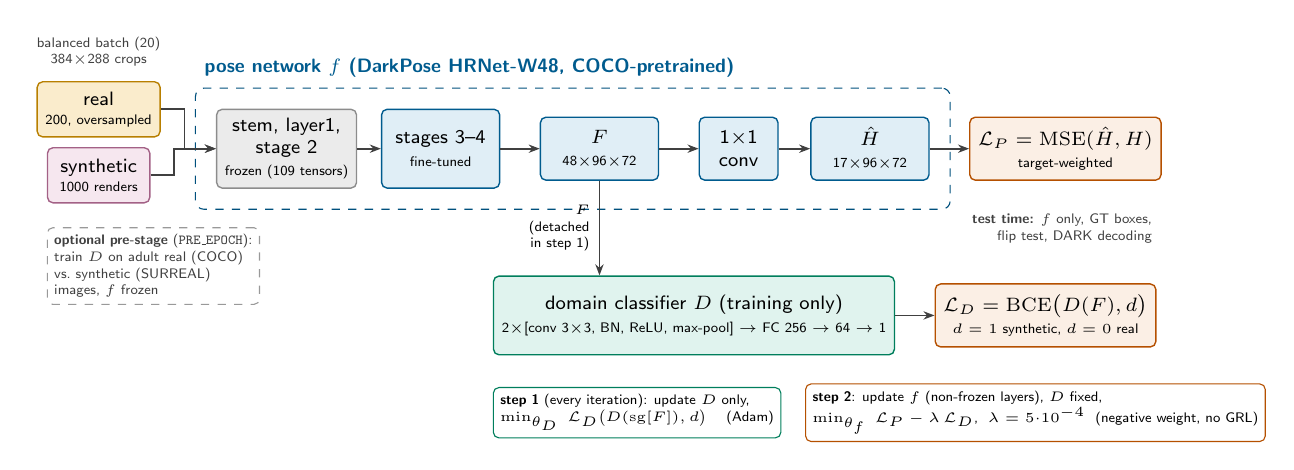
\begin{tikzpicture}[
  font=\sffamily\scriptsize,
  >={Stealth[length=4pt]},
  blk/.style={draw, rounded corners=2pt, align=center, minimum height=10mm, inner sep=3pt, line width=0.5pt},
  pose/.style={blk, fill=poseC!12, draw=poseC!80!black},
  froz/.style={blk, fill=black!8, draw=black!45, pattern color=black!18},
  dom/.style={blk, fill=domC!12, draw=domC!80!black},
  loss/.style={blk, fill=lossC!10, draw=lossC!85!black, minimum height=8mm},
  data/.style={blk, minimum height=7mm, minimum width=13mm},
  note/.style={align=left, text=black!75, font=\sffamily\tiny},
  flow/.style={->, line width=0.6pt, draw=black!75},
  grad/.style={->, line width=0.9pt, densely dashed},
]
% ---- inputs ---------------------------------------------------------------------------------
\node[data, fill=realC!20, draw=realC!80!black] (real) at (0,0.45) {real\\[-1pt]{\tiny 200, oversampled}};
\node[data, fill=synC!18, draw=synC!80!black, below=1.2mm of real] (syn) {synthetic\\[-1pt]{\tiny 1000 renders}};
\node[note, above=0.6mm of real, align=center] (inlab) {balanced batch (20)\\384$\times$288 crops};
% ---- pose network -----------------------------------------------------------------------------
\node[froz, right=7mm of real.south east, anchor=south west, yshift=-6.5mm, minimum width=16mm] (frozen)
  {stem, layer1,\\stage 2\\{\tiny frozen (109 tensors)}};
\node[pose, right=3mm of frozen, minimum width=15mm] (trainable) {stages 3--4\\{\tiny fine-tuned}};
\node[pose, right=5mm of trainable, minimum width=15mm, minimum height=8mm] (feat)
  {$F$\\{\tiny 48$\times$96$\times$72}};
\node[pose, right=5mm of feat, minimum width=10mm, minimum height=8mm] (head) {1$\times$1\\conv};
\node[pose, right=4mm of head, minimum width=15mm, minimum height=8mm] (hm) {$\hat H$\\{\tiny 17$\times$96$\times$72}};
\node[loss, right=5mm of hm, minimum width=19mm] (lp) {$\mathcal{L}_P=\mathrm{MSE}(\hat H, H)$\\{\tiny target-weighted}};
\begin{scope}[on background layer]
  \node[draw=poseC!70!black, dashed, rounded corners=3pt, fit=(frozen)(trainable)(feat)(head)(hm), inner sep=2.6mm,
        label={[font=\sffamily\scriptsize\bfseries, text=poseC!80!black, anchor=south west]north west:pose network $f$ (DarkPose HRNet-W48, COCO-pretrained)}] (posebox) {};
\end{scope}
\draw[flow] (real.east) -- ++(3mm,0) |- (frozen.west);
\draw[flow] (syn.east) -- ++(3mm,0) |- (frozen.west);
\draw[flow] (frozen) -- (trainable);
\draw[flow] (trainable) -- (feat);
\draw[flow] (feat) -- (head);
\draw[flow] (head) -- (hm);
\draw[flow] (hm) -- (lp);
% ---- domain classifier -------------------------------------------------------------------------
\node[dom, below=12mm of feat.south, anchor=north, xshift=12mm, minimum width=34mm] (dc)
  {domain classifier $D$ (training only)\\{\tiny 2$\times$[conv 3$\times$3, BN, ReLU, max-pool] $\to$ FC 256 $\to$ 64 $\to$ 1}};
\node[loss, right=5mm of dc, minimum width=27mm] (ld)
  {$\mathcal{L}_D=\mathrm{BCE}\big(D(F), d\big)$\\{\tiny $d=1$ synthetic, $d=0$ real}};
\draw[flow] (feat.south) -- node[left, font=\sffamily\tiny, align=right] {$F$\\(detached\\in step 1)} (feat.south |- dc.north);
\draw[flow] (dc) -- (ld);
% ---- the two alternating updates -------------------------------------------------------------
\node[draw=domC!80!black, fill=white, rounded corners=2pt, align=left, inner sep=2.5pt, font=\sffamily\tiny,
      below=4mm of dc.south west, anchor=north west] (s1)
  {\textbf{step 1} (every iteration): update $D$ only,\\ $\min_{\theta_D}\ \mathcal{L}_D\big(D(\mathrm{sg}[F]), d\big)$ \quad (Adam)};
\node[draw=lossC!85!black, fill=white, rounded corners=2pt, align=left, inner sep=2.5pt, font=\sffamily\tiny,
      right=3mm of s1] (s2)
  {\textbf{step 2}: update $f$ (non-frozen layers), $D$ fixed,\\ $\min_{\theta_f}\ \mathcal{L}_P-\lambda\,\mathcal{L}_D$, \ $\lambda=5{\cdot}10^{-4}$ \ (negative weight, no GRL)};
% ---- pre-stage and test-time notes -------------------------------------------------------------
\node[note, draw=black!40, dashed, rounded corners=2pt, inner sep=2.5pt, anchor=north west]
  at ([yshift=-3mm]syn.south west) (pre)
  {\textbf{optional pre-stage} (\texttt{PRE\_EPOCH}):\\train $D$ on adult real (COCO)\\vs.\ synthetic (SURREAL)\\images, $f$ frozen};
\node[note, anchor=north east, align=right] at ([yshift=-3mm]lp.south east)
  {\textbf{test time:} $f$ only, GT boxes,\\flip test, DARK decoding};
\end{tikzpicture}
}
  \caption[FiDIP as released]{FiDIP as released (DarkPose HRNet-W48), from \code{lib/models/adaptive_pose_hrnet.py} and \code{lib/core/function.py}. Step~1 of each iteration updates $D$ on detached stage-4 features. Step~2 updates the pose network with $\mathcal{L}_P-\lambda\mathcal{L}_D$, implemented as a negative loss weight. Only the pose network runs at test time.}
  \label{fig:fidip}
\end{figure}

\begin{table}[t]
\centering\small
\caption[FiDIP: paper vs.\ released code vs.\ our reproduction]{FiDIP as described in the paper (arXiv v5), as released (code and \code{w48_384x288_adam_lr1e-3_infant.yaml} at \texttt{a76b4f4}), and as we ran it.}
\label{tab:paper-vs-code}
\begin{adjustbox}{max width=\linewidth}
\begin{tabular}{@{}p{0.16\linewidth}p{0.22\linewidth}p{0.35\linewidth}p{0.25\linewidth}@{}}
\toprule
Aspect & Paper~\citep{huang2021fidip} & Released code / config~\citep{fidipcode} & Our reproduction\\
\midrule
Initialisation of $f$ & COCO-pretrained DarkPose & none unless \code{TRAIN.CHECKPOINT} is passed (random init) & COCO DarkPose \code{w48_384x288.pth}\\
$\lambda$ & $5{\cdot}10^{-4}$ & $0$ (infant yaml); $5{\cdot}10^{-4}$ only in \code{_custom.yaml} & $5{\cdot}10^{-4}$; $0$ as the fine-tune ablation\\
Optimiser, LR & Adam, $10^{-3}$ & Adam, $10^{-4}$, constant (LR steps at epochs 40 and 200 are never reached); $10^{-3}$ in \code{_custom.yaml} & released yaml; paper recipe as one extra attempt\\
Epochs / batch & 100 / 64 & 20 / 20 & released yaml\\
Adversarial update & gradient reversal layer & alternating updates with a negative loss weight; no GRL module & as released\\
Domain classifier & three FC layers & 2$\times$[conv3$\times$3, BN, ReLU, max-pool] + FC 256--64--1 on the 48-channel stage-4 high-resolution branch & as released\\
Classifier pre-stage & 1 epoch, batch 128; 1904 COCO vs.\ 2000 SURREAL adults & \code{PRE_EPOCH} 0 (infant yaml), 10 (\code{_custom.yaml}); the adult set (2029 real + 2028 synthetic) is said to be ``on request'' but ships in \code{syrip_for_train.zip} & \code{PRE_EPOCH} 10 on the shipped adult set\\
Frozen layers & Res1--3 (ResNet ablation) & first 109 parameter tensors (stem, \code{layer1}, stage 2) & as released\\
Real/synthetic balance & domain-dependent loss scale $S(I_i)$ & balanced sampler (200 real oversampled to 1000, interleaved, no reshuffle between epochs); unweighted loss & as released\\
Checkpoint selection & not stated & best Test100 AP, checked every epoch & best Val400 AP epoch\\
\bottomrule
\end{tabular}
\end{adjustbox}
\end{table}

\subsection{Published results and where the headroom is}\label{sec:published}

\Cref{tab:published} copies the published Test100 numbers.
With one infant and one detection per image, the true positives at a stricter OKS threshold are a subset of those at a looser one, so AP$_t$ cannot increase with $t$.
DarkPose + FiDIP reports AP$_{50}$ = AP$_{75}$ = 98.5, so all six thresholds from 0.50 to 0.75 score 98.5. The four strict thresholds then average
\[
\text{\APstrict}=(10\times93.6-6\times98.5)/4\approx86.3 .
\]
The same calculation gives 84.0 for DarkPose + Finetune (92.7 AP, also 98.5/98.5).
FiDIP's 0.9-point gain therefore lies entirely at strict thresholds, and so must any further gain. \Cref{sec:eval} shows that 98.5 is essentially a perfect score at loose thresholds on this test set.

\begin{table}[t]
\centering\small
\caption{Published SyRIP Test100 results~\citep{huang2021fidip,fidipcode}: COCO-pretrained (``Base''), fine-tuned on SyRIP, and FiDIP. The published baseline of this report is DarkPose + FiDIP, which also reports AP$_{50}$ = AP$_{75}$ = 98.5.}
\label{tab:published}
\begin{tabular}{@{}llcccc c@{}}
\toprule
Method & Backbone & Input & Base AP & + Finetune AP & + FiDIP AP & AR (FiDIP)\\
\midrule
SimpleBaseline & ResNet-50 & 384$\times$288 & 82.4 & 90.1 & 91.1 & 92.6\\
DarkPose & HRNet-W48 & 384$\times$288 & 88.5 & 92.7 & \textbf{93.6} & 94.6\\
Pose-MobileNet & MobileNetV2~\citep{sandler2018mobilenetv2} & 224$\times$224 & 46.5 & 78.9 & 79.2 & 84.1\\
\bottomrule
\end{tabular}
\end{table}

\subsection{Related work on SyRIP}\label{sec:related}

We found no later paper that beats 93.6 on Test100 with GT boxes. Later work on SyRIP uses other protocols:
\begin{itemize}[leftmargin=*]
  \item zero-shot adult models with \emph{detected} boxes on the 500 real test images (ViTPose best, at 41.9~AP)~\citep{gama2025seven};
  \item unsupervised adaptation measured by PCK~\citep{bose2025shift};
  \item 3D pose on Test100~\citep{huang2023symmetry,zhou2024zedoi};
  \item cross-dataset checks~\citep{grafton2025neonatal,jahn2025comparison}.
\end{itemize}
AggPose~\citep{cao2022aggpose} and InfantNet~\citep{hui2026infantnet} use their own, larger datasets.

\section{Implementation}\label{sec:impl}

\subsection{Compute and agentic workflow}\label{sec:workflow}

\paragraph{Compute.} Training and evaluation ran under Slurm on Northeastern's Explorer cluster~\citep{explorerdocs}:
\begin{itemize}[leftmargin=*]
  \item \code{gpu} (H200/A100, 8\,h limit) for training;
  \item \code{sharing} (1\,h) for smoke tests and evaluations;
  \item \code{short} for CPU jobs.
\end{itemize}
Datasets, environments and checkpoints stay on \code{/scratch}; only code, metrics, predictions and figures travel to the laptop, which had about 7\,GB free.

\paragraph{Agents.} Claude Code~\citep{claudecode}, running Claude Opus 5.5, acted as an \emph{orchestrator} (\cref{fig:workflow}). After the student approved a written plan, it launched four parallel workers, each with a self-contained brief:
\begin{itemize}[leftmargin=*]
  \item \emph{repro}: data, environments, released checkpoints and retraining;
  \item \emph{improve}: MMPose experiments;
  \item \emph{analysis}: the evaluator, statistics, figures and generated tables;
  \item \emph{report}: this document and the README.
\end{itemize}
A fresh-context reviewer checks the final state against the rubric.

\paragraph{Live files.} The orchestrator owns three of them:
\begin{itemize}[leftmargin=*]
  \item \code{SKILL.md}: how to operate the cluster;
  \item \code{AGENT.md}: the lab notebook of asks, attempts, failures and dated decisions D1, D2, \dots;
  \item \code{MANIFEST.md}: datasets, checkpoints, configs, and the run behind every number.
\end{itemize}
Workers log commands, job IDs and errors in \code{notebook/<stream>.md}, and register runs in \code{results/registry.csv}.

\paragraph{Shared rules.} All agents load \code{CLAUDE.md}, which requires:
\begin{itemize}[leftmargin=*]
  \item no compute on login nodes;
  \item no selection on Test100;
  \item one evaluator for every number;
  \item secrets only in a git-ignored \code{.env};
  \item timestamps from \code{date}.
\end{itemize}

\paragraph{Cluster loop.} The agent connects with \code{ssh -o BatchMode=yes -o ConnectTimeout=15} and wraps slow login-node commands in \code{timeout}, so failures surface quickly. For each job it:
\begin{enumerate}[leftmargin=*]
  \item pushes code with tar over ssh;
  \item submits an \code{sbatch} script, smoke-tested first on \code{sharing};
  \item polls \code{squeue}, \code{sacct} and the logs;
  \item pulls back only small artifacts.
\end{enumerate}
Each run's directory \code{runs/<RUN_ID>/} holds its resolved config, logs, predictions, evaluator outputs, and a \code{run.json} with the commit and tree SHAs, Slurm job ID, node, GPU, seed and checkpoint SHA256.

\begin{figure}[t]
  \centering
  \resizebox{0.92\linewidth}{!}{% Agentic workflow: human <-> orchestrator <-> worker agents, and the agent <-> Explorer/Slurm loop.
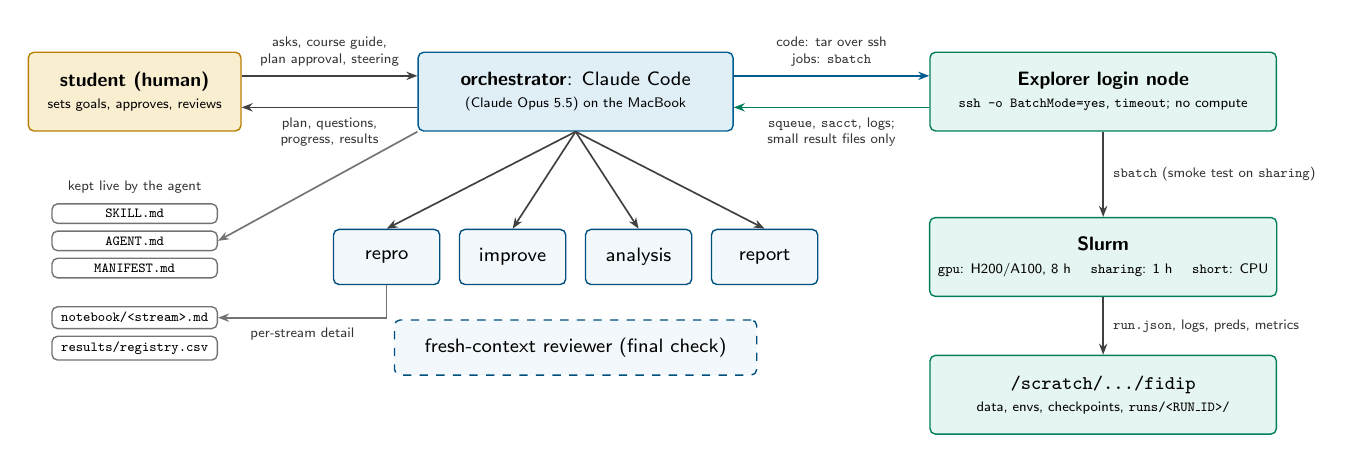
\begin{tikzpicture}[
  font=\sffamily\scriptsize,
  >={Stealth[length=4pt]},
  box/.style={draw, rounded corners=2pt, align=center, inner sep=3pt, line width=0.5pt},
  human/.style={box, fill=realC!18, draw=realC!80!black, minimum width=27mm, minimum height=10mm},
  agent/.style={box, fill=poseC!12, draw=poseC!80!black, minimum width=40mm, minimum height=10mm},
  worker/.style={box, fill=poseC!5, draw=poseC!70!black, minimum width=13.5mm, minimum height=7mm},
  doc/.style={box, fill=white, draw=black!55, minimum width=21mm, font=\ttfamily\tiny, inner sep=2pt},
  clus/.style={box, fill=domC!10, draw=domC!80!black, minimum width=44mm, minimum height=10mm},
  flow/.style={->, line width=0.6pt, draw=black!75},
  lab/.style={font=\sffamily\tiny, text=black!80, align=center},
]
% ---- top row: human -- orchestrator -- cluster login ---------------------------------------
\node[human] (human) at (0,0) {\textbf{student (human)}\\{\tiny sets goals, approves, reviews}};
\node[agent] (orch) at (5.6,0) {\textbf{orchestrator}: Claude Code\\{\tiny (Claude Opus 5.5) on the MacBook}};
\node[clus] (login) at (12.3,0) {\textbf{Explorer login node}\\{\tiny \texttt{ssh -o BatchMode=yes}, \texttt{timeout}; no compute}};
\draw[flow] ([yshift=2mm]human.east) -- node[lab, above] {asks, course guide,\\plan approval, steering} ([yshift=2mm]orch.west);
\draw[flow] ([yshift=-2mm]orch.west) -- node[lab, below] {plan, questions,\\progress, results} ([yshift=-2mm]human.east);
\draw[flow, poseC!80!black] ([yshift=2mm]orch.east) -- node[lab, above] {code: tar over ssh\\jobs: \texttt{sbatch}} ([yshift=2mm]login.west);
\draw[flow, domC!80!black] ([yshift=-2mm]login.west) -- node[lab, below] {\texttt{squeue}, \texttt{sacct}, logs;\\small result files only} ([yshift=-2mm]orch.east);
% ---- second row: workers, Slurm ---------------------------------------------------------------
\node[worker] (w1) at (3.2,-2.1) {repro};
\node[worker] (w2) at (4.8,-2.1) {improve};
\node[worker] (w3) at (6.4,-2.1) {analysis};
\node[worker] (w4) at (8.0,-2.1) {report};
\foreach \w in {w1,w2,w3,w4} \draw[flow] (orch.south) -- (\w.north);
\node[worker, dashed, minimum width=46mm] (rev) at (5.6,-3.25) {fresh-context reviewer (final check)};
\node[clus] (slurm) at (12.3,-2.1) {\textbf{Slurm}\\{\tiny \texttt{gpu}: H200/A100, 8 h \quad \texttt{sharing}: 1 h \quad \texttt{short}: CPU}};
\node[clus] (scratch) at (12.3,-3.85) {\textbf{\texttt{/scratch/.../fidip}}\\{\tiny data, envs, checkpoints, \texttt{runs/<RUN\_ID>/}}};
\draw[flow] (login) -- node[lab, right] {\texttt{sbatch} (smoke test on \texttt{sharing})} (slurm);
\draw[flow] (slurm) -- node[lab, right] {\texttt{run.json}, logs, preds, metrics} (scratch);
% ---- left column: the live files -------------------------------------------------------------
\node[doc] (skill) at (0,-1.55) {SKILL.md};
\node[doc, below=0.8mm of skill] (agentmd) {AGENT.md};
\node[doc, below=0.8mm of agentmd] (manifest) {MANIFEST.md};
\node[doc, below=3.5mm of manifest] (nb) {notebook/<stream>.md};
\node[doc, below=0.8mm of nb] (reg) {results/registry.csv};
\node[lab, anchor=south] at (skill.north) {kept live by the agent};
\draw[flow, black!55] (orch.south west) -- (agentmd.east);
\draw[flow, black!55] (w1.south) |- node[lab, pos=0.75, below] {per-stream detail} (nb.east);
\end{tikzpicture}
}
  \caption{Agentic workflow. The student sets goals, supplies the course material and approves the plan. The orchestrator keeps the three live files current and delegates to parallel workers. All compute goes through Slurm, and only small artifacts return to the laptop.}
  \label{fig:workflow}
\end{figure}

\subsection{Environments and compatibility patches}\label{sec:env}

\paragraph{Environments.} The upstream \code{fidip_env.yml} cannot be built: its pip stage pins \code{grpcio==1.48.2}, which has no Python~3.12 wheel, and \code{mkl-*} packages with no wheels. We built three environments instead:
\begin{itemize}[leftmargin=*]
  \item \emph{FiDIP:} pip-only, Python~3.12, PyTorch~2.3.1 (CUDA~12.1), NumPy~1.26.4, with every imported package pinned to the yml's version.
  \item \emph{MMPose:} Python~3.10, PyTorch~2.1.2, MMEngine~0.10.7, MMCV~2.1.0, MMPretrain~1.2.0 and MMPose~1.3.2~\citep{mmpose2020}, from conda-forge, with \code{numpy<2} and \code{opencv-python<4.12}.
  \item \emph{Analysis:} CPU-only, with the same NumPy and pycocotools pins as FiDIP.
\end{itemize}
Package lists are in \code{envs/} and checkpoint hashes in \code{MANIFEST.md}.

\paragraph{Upstream patches.} \Cref{app:patches} lists six upstream traps and our patches.
The most consequential trap, the README training command, needs no code change: \code{TRAIN.CHECKPOINT} and \code{TRAIN.LAMBDA} are passed on the command line.
The course guide's \code{gpu_test.py}, \code{tools/demo.py} and \code{tools/streamlit_demo.py} (and \code{fidip_simple.yml}) do not exist upstream. We wrote the GPU check and both demos from the guide's documented interface.

\subsection{Data preparation and the split protocol}\label{sec:data}

\paragraph{Download.} A Slurm job (\code{scripts/get_data.sh}):
\begin{enumerate}[leftmargin=*]
  \item downloads both public SyRIP archives, which needed no password;
  \item verifies their SHA256;
  \item extracts them on a compute node, because the login node killed \code{unzip};
  \item checks file counts against the archives;
  \item builds the upstream layout from symlinks and writes the split files.
\end{enumerate}
The adult \code{train_pre_infant} set (2029 real and 2028 synthetic images), described upstream as available on request, ships inside \code{syrip_for_train.zip}, so the classifier pre-stage can be run faithfully.
\code{SyRIP.zip}'s \code{images/train_infant/} also holds 300 unannotated real images, 199 of them byte-identical to validate500 images. We use only images listed in an annotation file.

\paragraph{Training labels.} Two annotation files cover the 1200 training images: the official \code{200R_1000S} file in \code{SyRIP.zip}, and \code{train_infant.json} in \code{syrip_for_train.zip}. They agree on the real images but differ on every synthetic one, because the second file carries MINI-RGBD labels:
\begin{itemize}[leftmargin=*]
  \item its source fields point to MINI-RGBD frames;
  \item eyes and ears are zeroed on most entries;
  \item some sizes and boxes do not fit the renders, with a median keypoint offset of 191\,px from the official labels (\code{notebook/repro.md}).
\end{itemize}
The images in the two archives are identical, except that the second archive's \code{validate_infant/test11.jpg} is a copy of \code{test24.jpg}.
Following the README literally therefore trains on mislabelled synthetic data and scores one test image against the wrong picture: the released checkpoint scores \res{sens.test11.ap}~AP on that archive's test images, against \res{rel.fidip.test.ap}~AP on the correct ones.
We use \code{SyRIP.zip}'s images and \code{200R_1000S} labels everywhere (D17); attempt R020 measures what the README-literal path costs.

\paragraph{Val400 (D15).} validate100 is a subset of validate500 (image ids 0--99, with identical files). \textbf{Val400} is validate500 ids 100--499 minus three images that duplicate Test100 images (two exact copies, one near-duplicate), which leaves 397 images.
Exact copies were found by file hash, and near-duplicates by a flip-aware perceptual hash with visual confirmation (\code{scripts/near_dups.py}).

\paragraph{Train/test overlap (D16).} Test100 images \code{test20}, \code{test42}, \code{test46} and \code{test50} are byte-identical to training images 73, 315, 272 and 340, and \code{test7} is a near-duplicate of training image 47.
We keep Test100 as shipped, for comparability with the published numbers (which carry the same overlap). As a sensitivity check we also report the 95-image \emph{Test100-clean} subset, where the released model's AP changes by \res{sens.clean.delta}.
Two further properties of the shipped GT need care.

\paragraph{Placeholder areas (D8).} Every validate500 annotation carries the same \code{area}, 2443298.48 ($\sqrt{\text{area}}\approx1563$\,px), and the training file carries another constant, 14232.77; validate100 instead uses $\text{area}=w\cdot h$ of its box.
Since OKS divides squared errors by the area (\cref{eq:oks}), the shipped Val400 makes almost any prediction look perfect: the released model scores \res{sens.area.const.ap}~AP on it.
We rebuilt Val400, validate500 and the framework-neutral training file with $\text{area}=w\cdot h$ from their own boxes, and left Test100 exactly as shipped. \code{scripts/make_splits.py} asserts this rule, and the evaluator refuses GT files whose areas are all identical.

\paragraph{Different boxes.} On the 100 shared images, validate100's boxes are a median \res{data.boxratio.pct}\% larger than validate500's, while the keypoints agree on 98 images; the other two were re-annotated. Val400 boxes are therefore tighter than Test100's, which means a smaller OKS scale and tighter crops (\cref{sec:thresholds}).

\paragraph{Protocol (D1).} \Cref{fig:protocol} summarises the protocol:
\begin{itemize}[leftmargin=*]
  \item Every choice of epoch, hyperparameter, backbone or recipe is made on Val400.
  \item A configuration reaches Test100 only after a commit lists it, with its Val400 evidence and checkpoint rule, in \code{results/PREREGISTRATION.md}.
  \item The final-evaluation script refuses unregistered or repeated runs, and checks the checkpoint SHA256 against \code{run.json}.
  \item The released checkpoints and the official-recipe retrains are reproduction targets, so they are evaluated on Test100 directly; the retrains' epochs are still chosen on Val400.
\end{itemize}

\paragraph{Why Val400.} It keeps the training data identical to the paper's, and it is almost twice as large as the real training set; cross-validation on the 200 real images could not match that without shrinking training.
It has two costs: Test500 is no longer clean, so we never report it, and Val400 is not the complex-pose subset, so it may rank models differently from Test100 (\cref{sec:thresholds}).

\begin{figure}[t]
  \centering
  \resizebox{0.92\linewidth}{!}{% Split and selection protocol: train on 200R+1000S, select on Val400, report once on Test100.
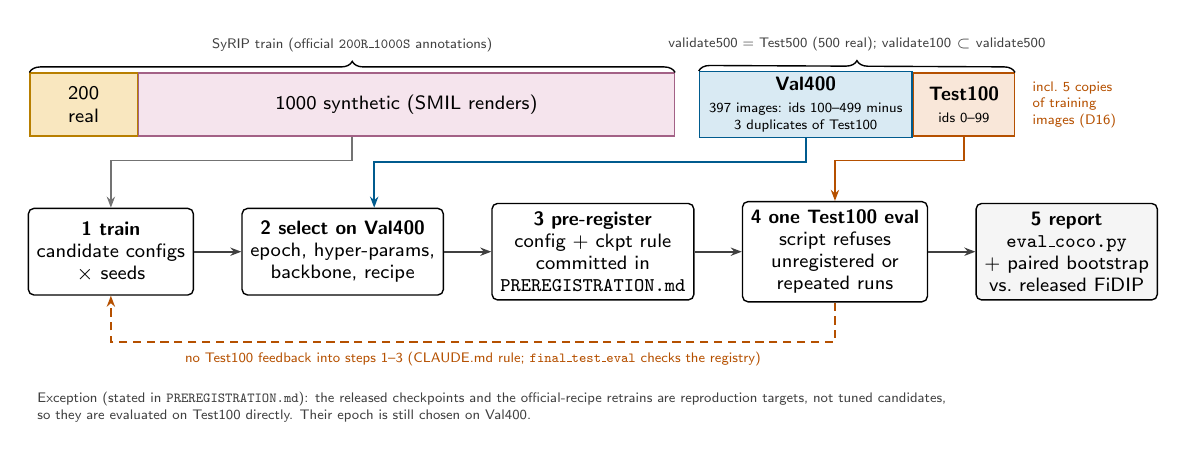
\begin{tikzpicture}[
  font=\sffamily\scriptsize,
  >={Stealth[length=4pt]},
  seg/.style={draw, line width=0.5pt, minimum height=8mm, align=center, inner sep=2pt},
  pstep/.style={draw, rounded corners=2pt, align=center, inner sep=3pt, line width=0.5pt, minimum height=11mm, fill=white},
  flow/.style={->, line width=0.6pt, draw=black!75},
  lab/.style={font=\sffamily\tiny, text=black!75, align=center},
]
% ---- the data bar (widths proportional to image counts: 1200 | 400 | 100) ----------------------
\def\u{0.0068}  % cm per image
\node[seg, fill=realC!25, draw=realC!80!black, minimum width=200*\u cm, anchor=west] (tr) at (0,0) {200\\real};
\node[seg, fill=synC!20, draw=synC!80!black, minimum width=1000*\u cm, anchor=west] (ts) at (tr.east) {1000 synthetic (SMIL renders)};
\node[seg, fill=poseC!15, draw=poseC!80!black, minimum width=397*\u cm, anchor=west, xshift=3mm] (val) at (ts.east)
  {\textbf{Val400}\\{\tiny 397 images: ids 100--499 minus}\\[-2pt]{\tiny 3 duplicates of Test100}};
\node[seg, fill=lossC!15, draw=lossC!85!black, minimum width=100*\u cm+6mm, anchor=west] (test) at (val.east)
  {\textbf{Test100}\\{\tiny ids 0--99}};
\draw[decorate, decoration={brace, amplitude=4pt}, line width=0.5pt] (tr.north west) -- node[lab, above=4pt] {SyRIP train (official \texttt{200R\_1000S} annotations)} (ts.north east);
\draw[decorate, decoration={brace, amplitude=4pt}, line width=0.5pt] (val.north west) -- node[lab, above=4pt] {validate500 = Test500 (500 real); validate100 $\subset$ validate500} (test.north east);
\node[lab, right=1mm of test.east, anchor=west, text=lossC!85!black, align=left] {incl.\ 5 copies\\of training\\images (D16)};
% ---- the procedure ----------------------------------------------------------------------------
\node[pstep, below=9mm of ts.south west, anchor=north west, xshift=-14mm] (s1)
  {\textbf{1 train}\\candidate configs\\$\times$ seeds};
\node[pstep, right=6mm of s1] (s2) {\textbf{2 select on Val400}\\epoch, hyper-params,\\backbone, recipe};
\node[pstep, right=6mm of s2] (s3) {\textbf{3 pre-register}\\config + ckpt rule\\committed in\\\texttt{PREREGISTRATION.md}};
\node[pstep, right=6mm of s3] (s4) {\textbf{4 one Test100 eval}\\script refuses\\unregistered or\\repeated runs};
\node[pstep, right=6mm of s4, fill=black!4] (s5) {\textbf{5 report}\\\texttt{eval\_coco.py}\\+ paired bootstrap\\vs.\ released FiDIP};
\draw[flow] (s1) -- (s2);
\draw[flow] (s2) -- (s3);
\draw[flow] (s3) -- (s4);
\draw[flow] (s4) -- (s5);
\draw[flow, black!55] ($(tr.south west)!0.5!(ts.south east)$) -- ++(0,-3mm) -| (s1.north);
\draw[flow, poseC!80!black] (val.south) -- ++(0,-3mm) -| ([xshift=4mm]s2.north);
\draw[flow, lossC!85!black] (test.south) -- ++(0,-3mm) -| (s4.north);
% ---- the forbidden edge ----------------------------------------------------------------------------
\draw[->, line width=0.6pt, lossC!85!black, densely dashed] (s4.south) -- ++(0,-5mm) -| node[pos=0.25, below, lab, text=lossC!85!black]
  {no Test100 feedback into steps 1--3 (CLAUDE.md rule; \texttt{final\_test\_eval} checks the registry)} (s1.south);
\node[lab, anchor=north west, align=left] at ([yshift=-11mm]s1.south west)
  {Exception (stated in \texttt{PREREGISTRATION.md}): the released checkpoints and the official-recipe retrains are reproduction targets, not tuned candidates,\\so they are evaluated on Test100 directly. Their epoch is still chosen on Val400.};
\end{tikzpicture}
}
  \caption{Split and selection protocol (bar widths proportional to image counts). Test100 is read once per pre-registered configuration, and nothing learned from it flows back into training or selection.}
  \label{fig:protocol}
\end{figure}

\subsection{One evaluator for every number}\label{sec:eval}

\paragraph{Pipeline.} Every metric comes from \code{eval/eval_coco.py} (v1.0) applied to a prediction JSON, and both frameworks take the same path:
\begin{enumerate}[leftmargin=*]
  \item a loader that accepts twelve prediction encodings;
  \item one rescoring rule, score $=\mathrm{mean}(c_k\,|\,c_k>0.2)$, which is upstream FiDIP's rule and MMPose's \code{bbox_keypoint} mode with a box score of 1 for GT boxes. It keeps the image ranking, and therefore AP, comparable;
  \item a verbatim port of upstream OKS-NMS, which is a no-op with one box per image;
  \item pycocotools 2.0.8 \code{COCOeval}~\citep{cocoapi}, with the COCO sigmas and the GT area.
\end{enumerate}
Besides the usual metrics it writes per-threshold AP, \APstrict{} and per-image OKS. It also writes per-keypoint errors normalised by $\sqrt{wh}$ of the GT box (the OKS scale on Test100), with PCK@\{0.05, 0.1, 0.2\}.

\paragraph{The annotation-id-0 artifact (D10).} In Test100, annotation ids equal image ids, so \code{test0.jpg} carries id~0. \code{COCOeval.evaluateImg} stores the matched GT id in \code{dtMatches}, and \code{accumulate} treats a stored 0 as ``unmatched''. The infant in \code{test0.jpg} can therefore never be a true positive, and its detection always counts as a false positive.
This caps AR at 0.99, and even a perfect model's AP at every threshold is
\[
\frac{r+0.99\,(100-r)}{101}\in[0.980,\,0.990],
\]
where $r$ is the rank of test0's score (unit-tested).
The published AP$_{50}$ = AP$_{75}$ = 98.5 falls inside this band, so on the 99 matchable images the published models are already perfect at loose thresholds. The near-constant AR$_{50}$ = 99.0 of the upstream table has the same cause.

The size of this penalty depends only on where test0's score ranks: between \res{sens.id0.min} and \res{sens.id0.max}~AP at realistic accuracy.
Our headline \texttt{paper} protocol keeps the ids as shipped, so it stays comparable with 93.6. A \texttt{fixed} protocol shifts the ids off 0. An improvement claim counts only if its paired CI excludes 0 under \emph{both} protocols, and every model's test0 rank is reported (D13). On Val400, which has no id~0, the two protocols coincide.
This is a property of the evaluation tooling, not an error in the published work: anyone scoring this file with pycocotools gets the same cap.

\paragraph{MMPose's evaluator.} MMPose's \code{CocoMetric} uses xtcocotools~\citep{xtcocotools}, which marks unmatched detections with $-1$. Its printed Test100 AP therefore equals our \texttt{fixed} protocol, \res{sens.xtcoco.delta}~AP away from \texttt{paper} on identical predictions.
Comparing it with 93.6 would overstate any gain, which is why only \code{eval_coco.py} numbers are compared (D2).

\paragraph{Verification and statistics.}
\begin{itemize}[leftmargin=*]
  \item \emph{Unit tests.} 24 tests cover the GT-as-prediction case, the id-0 ceiling, noise monotonicity, encoding invariance, rescoring, OKS against \code{COCOeval} internals, and NMS against upstream (\cref{app:tests}).
  \item \emph{Cross-check.} On the released checkpoint's predictions, upstream's own test script reports \res{rel.fidip.test.ap.upstream}~AP and ours \res{rel.fidip.test.ap}~AP.
  \item \emph{Uncertainty.} \code{eval/bootstrap_ci.py} resamples the 100 test images ($B=\res{boot.n}$), recomputes AP exactly, and reports paired 95\% percentile CIs of seed-averaged AP differences and Holm-adjusted one-sided $p$-values~\citep{efron1993bootstrap}.
\end{itemize}

\section{Reproduction results}\label{sec:repro}

\subsection{Released checkpoints}\label{sec:released}

\paragraph{Setup.} We evaluated three checkpoints under their released test settings (GT boxes, flip test, DARK post-processing), with predictions scored by \code{eval_coco.py} (\cref{tab:repro}, upper block):
\begin{itemize}[leftmargin=*]
  \item \code{hrnet_fidip.pth}, DarkPose + FiDIP;
  \item \code{mobile_fidip.pth}, Pose-MobileNet + FiDIP;
  \item the COCO-only DarkPose \code{w48_384x288.pth} that FiDIP starts from.
\end{itemize}

\paragraph{Results.} The released FiDIP model scores \res{rel.fidip.test.ap}~AP under the \texttt{paper} protocol (\res{rel.fidip.test.diffpub} from the published 93.6), and \res{rel.fidip.test.ap.fixed}~AP under \texttt{fixed}. The individual metrics, against the published values:
\begin{itemize}[leftmargin=*]
  \item AP$_{50}$ \res{rel.fidip.test.ap50} and AP$_{75}$ \res{rel.fidip.test.ap75} (98.5 each);
  \item AR \res{rel.fidip.test.ar} (94.6);
  \item \APstrict{} \res{rel.fidip.test.apstrict} (86.3 implied, \cref{sec:published}).
\end{itemize}
The released Pose-MobileNet scores \res{rel.mobile.test.ap}~AP (published 79.2), and the COCO-only DarkPose \res{zs.darkpose.test.ap}~AP (published 88.5).

\interp{Does the released checkpoint reproduce 93.6 within what 100 test images allow? If not, does AP$_{50}$/AP$_{75}$ or \APstrict{} explain the gap, and does upstream's printed AP agree (\cref{sec:eval})?}

\begin{table}[t]
  \centering\small
  \caption[Reproduction on Test100 and Val400]{Reproduction on SyRIP Test100 (\texttt{paper} protocol, GT boxes, flip test) and Val400. \emph{Upper block:} released checkpoints scored by \code{eval_coco.py}. \emph{Lower block:} retrains with the released recipe from COCO DarkPose weights (mean $\pm$ s.d.\ over seeds, epochs selected on Val400). ``Publ.'' is the published AP~\citep{huang2021fidip,fidipcode}.}
  \label{tab:repro}
  \GenTable{tab_reproduction}{released checkpoints and retrains vs.\ published}
\end{table}

\subsection{Retraining FiDIP and the fine-tuning ablation}\label{sec:retrain}

\paragraph{Recipe.} We retrained with the released code and yaml, adding two command-line overrides (D5): \code{TRAIN.CHECKPOINT} set to the COCO DarkPose weights, and \code{TRAIN.LAMBDA} set to the paper's $5{\cdot}10^{-4}$.
The classifier pre-stage runs for 10 epochs (\code{PRE_EPOCH}, as in \code{_custom.yaml}) on the shipped adult set. The model is evaluated on Val400 after every epoch, and the best epoch is kept.
To isolate domain adaptation, we also ran the same recipe with $\lambda=0$, which is the paper's ``DarkPose + Finetune'' row. Each arm has \res{rt.seeds} seeds.

Because the paper's recipe differs from the yaml (\cref{tab:paper-vs-code}), we also ran two extra attempts, listed in \cref{sec:attempts}:
\begin{itemize}[leftmargin=*]
  \item the paper's recipe once (Adam $10^{-3}$, 100 epochs, batch 64), D12;
  \item a single-seed $\lambda$ sweep on Val400, D9.
\end{itemize}

\paragraph{Results.} On Test100, FiDIP scores \resms{rt.fidip.test.ap}~AP and fine-tuning \resms{rt.ft.test.ap}~AP. On Val400 they score \resms{rt.fidip.val.ap} and \resms{rt.ft.val.ap}.
The seed-averaged difference on Test100 is \res{rt.delta.test.ap}~AP, with 95\% CI [\res{rt.delta.test.ci.lo}, \res{rt.delta.test.ci.hi}] and one-sided $p=\res{rt.delta.test.p}$ (\cref{tab:repro}, lower block).

\interp{Is FiDIP's published 0.9-AP gain over fine-tuning (92.7 to 93.6) reproduced, and is it distinguishable from seed and sampling noise at $n=100$? How does the retrain compare with the released checkpoint?}

\subsection{Training dynamics: over- and underfitting}\label{sec:curves}

\paragraph{What we monitor.} As the course guide asks, every run logs the training loss and the Val400 AP after each epoch, and FiDIP runs also log the domain-classifier loss (\cref{fig:curves}).
Out of \res{rt.epochs} epochs, the median Val400-selected epoch is \res{rt.fidip.bestepoch} for FiDIP and \res{rt.ft.bestepoch} for fine-tuning.

\paragraph{Risk factors.} Two features of the data invite overfitting: there are only 200 real images, each seen about five times per epoch through the balanced sampler, and the batch order never changes between epochs. The released recipe counteracts this with a low constant LR ($10^{-4}$) and frozen early layers.

\begin{figure}[t]
  \centering
  \GenFigure[width=\linewidth]{curves_fidip}{per-epoch training loss, Val400 AP (and domain loss) for the FiDIP and fine-tune retrains, all seeds}
  \caption{Retrain curves: training loss and Val400 AP per epoch for all seeds, with the Val400-selected epoch marked. Test100 was never evaluated per epoch.}
  \label{fig:curves}
\end{figure}

\interp{Does Val400 AP plateau or fall while the training loss keeps decreasing (overfitting)? Is it still rising at the last epoch (underfitting, which would argue for the paper's longer schedule)? How does the domain loss behave at $\lambda=5{\cdot}10^{-4}$?}

\section{Improving on FiDIP}\label{sec:improve}

\subsection{Hypothesis and method}\label{sec:method}

\paragraph{Hypothesis.} The published model is already essentially perfect at OKS 0.50--0.75 on the 99 matchable images (\cref{sec:published,sec:eval}). Any gain must therefore come from more precise localisation, which \APstrict{} measures.
Two standard levers act on precision: backbone capacity with stronger pre-training, and higher input resolution, which gives finer heatmaps.
We test both with ViTPose~\citep{xu2022vitpose}. In the MMPose model zoo~\citep{mmpose2020}, its COCO checkpoints score 78.2~AP (L) and 78.8~AP (H), against 77.2~AP for HRNet-W48 + DARK at $384{\times}288$ (COCO val2017, detected boxes).

\paragraph{Arms.} All improvement runs use MMPose~1.3.2.
\begin{itemize}[leftmargin=*]
  \item The \emph{control} is HRNet-W48 + DARK at $384{\times}288$, the MMPose counterpart of FiDIP's network.
  \item The \emph{resolution arm} is ViTPose-L at $256{\times}192$ and $384{\times}288$.
  \item The \emph{capacity arm} is ViTPose-H at $384{\times}288$.
\end{itemize}

\paragraph{What is held fixed.} Every arm uses the same training data (200 real + 1000 synthetic, official labels) and FiDIP's 1:1 real:synthetic mix, in which each real image appears five times per 2000-sample epoch. Every arm also shares the epoch budget, warm-up and LR decay, MMPose's COCO augmentation, GT boxes, flip test, and per-epoch Val400 checkpoint selection.

\paragraph{What varies.} Only what each family needs: HRNet uses Adam, while ViT uses AdamW with layer-wise LR decay and drop-path. Batch size and codec (DARK versus UDP) also differ.
We therefore compare backbone families, each with its standard optimiser, rather than doing a pure weight swap.

Starting from FiDIP's nominal LR of $10^{-4}$, we explored recipe knobs (LR, rotation range, schedule, EMA) on Val400 only (\cref{tab:attempts}); the resolved settings are in \cref{tab:hparams}.
Besides SyRIP, the only pose data are the COCO checkpoints. We excluded models whose pre-training adds other pose datasets.

\subsection{Controlled comparison and ablations}\label{sec:backbone}\label{sec:ablations}

\Cref{tab:backbone} gives Val400 AP (mean $\pm$ s.d.\ over seeds) and \APstrict{} per arm. The MMPose control reaches \resms{imp.control.val.ap}~AP, and the configuration finally pre-registered, \res{best.name}, reaches \resms{best.val.ap}~AP.

\Cref{tab:ablations} changes one factor at a time against a stated default, on Val400 only:
\begin{itemize}[leftmargin=*]
  \item real-only versus real + synthetic training data;
  \item the rotation range;
  \item flip testing;
  \item the FiDIP weight $\lambda$.
\end{itemize}

\begin{table}[t]
  \centering\small
  \caption{Controlled comparison under one MMPose recipe (Val400, mean $\pm$ s.d.\ over seeds). Test100 is shown only for pre-registered runs (otherwise ---). GPU-hours are per training run.}
  \label{tab:backbone}
  \GenTable{tab_backbone}{backbone $\times$ input-size comparison on Val400}
\end{table}

\begin{table}[t]
  \centering\small
  \caption{Ablations, one factor at a time, on Val400. $\Delta$ is relative to the default row.}
  \label{tab:ablations}
  \GenTable{tab_ablations}{one-factor ablations on Val400}
\end{table}

\interp{Name the Val400 winner. Which matters more, resolution (L at $256{\times}192$ vs.\ $384{\times}288$) or capacity (L vs.\ H)? Does the gain appear in \APstrict{} as hypothesised? Is synthetic data still useful for a strong backbone, and what do rotation, flip-TTA and $\lambda$ contribute?}

\subsection{All attempts}\label{sec:attempts}

The course asks for the accuracy of \emph{every} attempt. \Cref{tab:attempts} lists all \res{att.n} in chronological order, including those that did not help:
\begin{itemize}[leftmargin=*]
  \item the reproduction variants;
  \item the domain-adaptation tweaks (the $\lambda$ sweep and the paper recipe);
  \item every backbone, resolution, augmentation and recipe change.
\end{itemize}
\res{att.nbetter} attempts beat the control's mean Val400 AP. Test100 values appear only for pre-registered runs.

\begin{table}[t]
  \centering\footnotesize
  \caption[Every attempt with its accuracy]{Every attempt with its Val400 accuracy and outcome, generated from \code{results/registry.csv}. Run IDs resolve to \code{runs/<RUN_ID>/} and to \code{MANIFEST.md}.}
  \label{tab:attempts}
  \GenTable{tab_attempts}{every attempt with its accuracy}
\end{table}

\subsection{Final evaluation: repeats and confidence intervals}\label{sec:final}

After the Val400 study, \res{best.name} was pre-registered at commit \res{best.prereg.commit}, with the checkpoint rule ``\res{best.ckptrule}''. It was then evaluated once on Test100 for each of its \res{best.seeds} seeds (\cref{tab:final}).
Differences are paired with the released FiDIP checkpoint on the same 100 images. The published 93.6 has no per-image predictions, so it cannot be paired.
The paired image bootstrap of the seed-averaged AP (\cref{sec:eval}) covers both test-sampling and seed variation. Following D13, the claim requires the CI to exclude 0 under both the \texttt{paper} and the \texttt{fixed} protocol (\cref{tab:boot}).

\begin{table}[t]
  \centering\small
  \caption{Final Test100 comparison (\texttt{paper} protocol). $\Delta$AP is paired with the released checkpoint on the same images (95\% percentile bootstrap CI, $B=\res{boot.n}$); $p$ is one-sided and Holm-adjusted. The published row is copied from~\citep{fidipcode}.}
  \label{tab:final}
  \GenTable{tab_final}{final Test100 comparison with bootstrap CIs}
\end{table}

\begin{table}[t]
  \centering\small
  \caption{Paired image-level bootstrap contrasts on Test100 under both protocols. ``Robust'' means the 95\% CI excludes 0 under both \texttt{paper} and \texttt{fixed} (D13); W/T/L counts per-image OKS wins, ties and losses.}
  \label{tab:boot}
  \GenTable{tab_boot}{bootstrap contrasts under both protocols}
\end{table}

\begin{keybox}{Published baseline vs.\ our result, and the exact evaluation conditions}
\textbf{Published baseline.} DarkPose + FiDIP, HRNet-W48, $384{\times}288$: \textbf{93.6~AP} on SyRIP Test100 (AP$_{50}$ 98.5, AP$_{75}$ 98.5, AR 94.6)~\citep{huang2021fidip,fidipcode}.

\textbf{The same model under our evaluator.} Released \code{hrnet_fidip.pth}: \res{rel.fidip.test.ap}~AP (\texttt{paper}), \res{rel.fidip.test.ap.fixed}~AP (\texttt{fixed}).

\textbf{Our result.} \res{best.name}: \textbf{\resms{best.test.ap}~AP} on Test100, mean $\pm$ s.d.\ over \res{best.seeds} seeds, \texttt{paper} protocol.
\begin{itemize}[leftmargin=12pt]
  \item Against the released checkpoint on the same images: $\Delta$AP $=$ \res{best.delta.ap}, 95\% CI [\res{best.delta.ci.lo}, \res{best.delta.ci.hi}], one-sided $p=\res{best.delta.p}$.
  \item Against the published 93.6: \res{best.vs.published}.
  \item Same contrast under the \texttt{fixed} protocol: \res{best.delta.fixed}, 95\% CI [\res{best.delta.fixed.ci.lo}, \res{best.delta.fixed.ci.hi}]. Robust under both protocols (D13): \textbf{\res{best.robust}}.
  \item \APstrict{}: \res{best.test.apstrict} (\res{best.delta.apstrict} against the released checkpoint). On Test100-clean: \res{best.test.clean.ap}~AP.
\end{itemize}

\textbf{Evaluation conditions}, identical for every compared row:
\begin{itemize}[leftmargin=12pt]
  \item \emph{Test set:} SyRIP \code{validate100} (= Test100), 100 real images exactly as distributed. Boxes, areas and annotation ids are unchanged, and the five images that duplicate training images are kept, as in the published evaluation; Test100-clean (95 images) is a sensitivity check.
  \item \emph{Training data:} 200 real + 1000 synthetic images, with the official \code{200R_1000S} labels. No Val400 or Test100 image was added to training.
  \item \emph{Inference:} GT person boxes, flip test \res{best.flip}, input \res{best.input}, one model per seed. Ensembles are reported separately.
  \item \emph{Metric:} \code{eval/eval_coco.py} v1.0, i.e.\ pycocotools 2.0.8 \code{COCOeval} (keypoints, COCO-17 sigmas, GT area, maxDets 20) after shared rescoring and OKS-NMS, with annotation id~0 kept as in the published numbers (\cref{sec:eval}). Claims must also hold under the \texttt{fixed} protocol. The test0 score rank is \res{best.test0rank} for our model and \res{rel.fidip.test0rank} for the released one.
  \item \emph{Selection:} epochs, hyperparameters and the configuration were chosen on Val400 only. The configuration was pre-registered at commit \res{best.prereg.commit} before its single Test100 evaluation, and no Test100 result fed back into any choice.
\end{itemize}
\end{keybox}

\interp{Two-sentence conclusion: is the improvement over the released checkpoint supported by the CI, and where does it come from (\APstrict{}, per-keypoint results in \cref{sec:analysis})? If the CI includes 0, say plainly that no improvement was established.}

\paragraph{Ensemble (secondary claim).} A coordinate ensemble across seeds (\code{eval/ensemble_preds.py}) was registered separately and is never mixed with single-model numbers. Its status is \res{ens.name}. When run, it scores \res{ens.test.ap}~AP, with a paired 95\% CI against the released checkpoint of [\res{ens.delta.ci.lo}, \res{ens.delta.ci.hi}].

\section{Analysis}\label{sec:analysis}

\subsection{Where AP is lost, and how Val400 relates to Test100}\label{sec:thresholds}

\paragraph{Per threshold.} \Cref{fig:thresholds} (left) plots Test100 AP at each OKS threshold, together with the \texttt{paper}-protocol ceiling of a perfect model (\cref{sec:eval}).
Every model sits on the ceiling up to $t=0.75$. They separate only above it: the released model's \APstrict{} is \res{rel.fidip.test.apstrict}.
On this test set, AP is decided by localisation precision, not by gross failures.

\paragraph{Val400 against Test100.} \Cref{fig:thresholds} (right) shows Val400 against Test100 AP. Across the \res{vt.n} runs with both, the Spearman rank correlation is \res{vt.spearman}, and Test100 exceeds Val400 by \res{vt.gap.mean}~AP on average.
Test100's looser boxes explain part of that gap (\cref{sec:released}). The ranking transfers reasonably even though Test100 was chosen for complex poses.

\begin{figure}[t]
  \centering
  \begin{minipage}[b]{0.63\linewidth}\centering
    \GenFigure[width=\linewidth]{oks_thresholds}{AP at OKS 0.50--0.95: released FiDIP, retrain, best config; paper-protocol ceiling band}
  \end{minipage}\hfill
  \begin{minipage}[b]{0.33\linewidth}\centering
    \GenFigure[width=\linewidth]{val_vs_test}{Val400 AP vs Test100 AP, one point per run that has both}
  \end{minipage}
  \caption{Left: Test100 AP at each OKS threshold, for the \texttt{paper} protocol (with the ceiling band of a perfect model under the id-0 artifact) and, in the second sub-panel, the \texttt{fixed} protocol. Right: Val400 against Test100 AP for every run evaluated on both sets.}
  \label{fig:thresholds}\label{fig:valtest}
\end{figure}

\paragraph{Evaluation choices.} \Cref{tab:sensitivity} (\cref{app:attempts}) holds the released model's predictions fixed and changes one evaluation choice at a time. Each choice moves AP by about as much as FiDIP's published gain over fine-tuning (0.9):
The matching protocol moves AP by \res{sens.id0.delta}, and moving test0's score rank alone swings the \texttt{paper} AP from \res{id0.rank.lo} to \res{id0.rank.hi}. Test100-clean moves it by \res{sens.clean.delta}, validate500's boxes give \res{sens.box.v500.ap} instead of \res{sens.box.v100.ap}, the misplaced \code{test11} costs \res{test11.delta}, and the placeholder area inflates Val400 to \res{sens.area.const.ap} from \res{rel.fidip.val.ap}.

\subsection{Per-keypoint accuracy and failure modes}\label{sec:perkp}\label{sec:failures}

\paragraph{Per keypoint.} \Cref{fig:perkp} (left) and \cref{tab:perkp} break the error down by joint. \textbf{Hips are by far the hardest joints}: their median error is more than twice that of any other group, and fewer than half fall within 5\% of the box scale.
This fits infant anatomy: hip centres are hidden under diapers and clothing, and legs are often flexed against the trunk. The paper likewise found the lower body hardest for adult-trained models~\citep{huang2021fidip}.
Heads and wrists are the most precise.

\paragraph{Failure modes.} \code{eval/taxonomy.py} assigns failure modes with unit-tested rules (\cref{tab:failures} in \cref{app:attempts} gives counts and exact criteria).
\textbf{Rotation dominates} (\cref{fig:perkp}, right): \res{fail.sideways.n} of the 100 infants lie sideways, with a mean OKS deficit of \res{fail.sideways.deficit}\% against \res{fail.upright.deficit}\% for upright infants. Left/right swaps are rare (\res{fail.lrswap.n} image, a back view), no prediction is a whole-body mirror, \res{fail.occl.n} images are heavily occluded and \res{fail.inverted.n} have an inverted torso.
The failures are mostly a matter of degree: sideways and partly hidden infants get somewhat imprecise joints, not catastrophic errors. That is consistent with AP being decided at strict thresholds.
\Cref{fig:qual} shows the worst Test100 cases.

\begin{figure}[t]
  \centering
  \begin{minipage}[b]{0.5\linewidth}\centering
    \GenFigure[width=\linewidth]{per_keypoint}{per-keypoint normalised error and PCK@0.05 (Test100)}
  \end{minipage}\hfill
  \begin{minipage}[b]{0.46\linewidth}\centering
    \GenFigure[width=\linewidth]{error_vs_orientation}{error vs torso orientation (Test100)}
  \end{minipage}
  \caption{Left: per-keypoint error on Test100, normalised by $\sqrt{wh}$ of the GT box (the OKS scale). Right: error by in-plane torso orientation; sideways infants carry most of the error.}
  \label{fig:perkp}
\end{figure}


\begin{figure}[t]
  \centering
  \GenFigure[width=\linewidth,height=0.2\textheight,keepaspectratio]{qual_failure}{overlay grid: worst Test100 cases}
  \caption{The lowest-OKS Test100 cases for the released FiDIP model, with GT and predictions overlaid (legend in the figure). The best cases are shown in \cref{fig:qualsucc}.}
  \label{fig:qual}
\end{figure}

\subsection{Inference demo}\label{sec:demo}

Part~6 of the course guide asks for two demos. The command-line demo \code{tools/demo.py} follows the guide's interface: \code{--cfg}, \code{--image}, \code{--model}, \code{--output}, and optionally \code{--conf-threshold} and \code{--output-size}; it also accepts \code{--video}.
\code{tools/streamlit_demo.py} lets a user upload an image, set the confidence threshold with a slider, and view keypoints with their confidences. Both were verified on the cluster, the Streamlit app through its AppTest harness and a live health check.

\Cref{fig:demo} (appendix) shows one practical lesson. The same image is processed with the GT box and with a detector box. Mean keypoint confidence drops from \res{demo.conf.gt} to \res{demo.conf.det}, so box quality matters as much as the pose model once GT boxes are gone.


\section{Limitations}\label{sec:limits}

\begin{itemize}[leftmargin=*]
  \item \textbf{A 100-image test set.} One image can move AP by about a point, and strong models' AP$_{50}$/AP$_{75}$ sit at the id-0 ceiling. Differences below about one AP are hard to establish (see \cref{tab:final}), and three seeds give only a rough estimate of seed variance.
  \item \textbf{One protocol.} Like the published work, we use GT person boxes. The numbers therefore say nothing about deployment with a person detector, where zero-shot adult models reach about 42~AP on SyRIP's real test images~\citep{gama2025seven}.
  \item \textbf{Selection-set mismatch.} Val400 is what remains of validate500 once the complex poses are removed, and its boxes are tighter than Test100's. It may favour models that do well on easier poses. The correlation in \cref{sec:thresholds} measures how well it transfers, but evaluating Test100 only once per configuration limits the number of such comparisons.
  \item \textbf{What ``reproduction'' means here.} Our retrains differ from the released code in three ways:
  \begin{itemize}[leftmargin=*]
    \item They select epochs on Val400, whereas the released loop selects on Test100. Test-set selection can only raise the reported test score, so a small shortfall of a Val400-selected retrain is expected and is not by itself a failed reproduction.
    \item The upstream README points training to \code{syrip_for_train.zip}, whose synthetic labels do not match the images (\cref{sec:data}). We used the official labels, and we cannot tell which file produced the published models.
    \item The paper's recipe differs from the config, and we ran the paper's recipe only once.
  \end{itemize}
  \item \textbf{Kept artifacts.} For comparability, the headline numbers keep two properties of the published evaluation:
  \begin{itemize}[leftmargin=*]
    \item the pycocotools id-0 artifact. The \texttt{fixed} numbers are closer to the true COCO AP, and claims must hold under both protocols;
    \item the five Test100 images that duplicate training images. They favour any model that memorises its training set, so the Test100-clean subset is reported alongside.
  \end{itemize}
  \item \textbf{Scope of the search.}
  \begin{itemize}[leftmargin=*]
    \item We tried ViTPose-L/H at two input sizes and a few recipe changes.
    \item We excluded backbones pre-trained on extra pose data.
    \item ViTPose with FiDIP-style adaptation was a stretch goal; its status is in \cref{tab:attempts}.
    \item Only comparisons within MMPose are controlled, because upstream and MMPose also differ in augmentation and training code.
  \end{itemize}
  \item \textbf{Expanded SyRIP.} Its 400 extra real training images are most likely validate500 \textbackslash{} validate100, which is our Val400. Training on them would consume the selection set and change the split, so it is out of scope under the same-split rule. A natural follow-up is to train on the expanded set, select by cross-validation, and report on Test100.
  \item \textbf{Agent-executed work.} An AI agent did most of the execution and made mistakes (\cref{sec:aiuse}). Tests, cross-checks, pre-registration and provenance records reduce the risk, but no safeguard is complete.
\end{itemize}

\section{Lessons learned}\label{sec:lessons}

\paragraph{Small-data evaluation.}
\begin{itemize}[leftmargin=*]
  \item \textbf{On 100 test images, evaluation details are as large as method effects.} The id-0 artifact, the evaluator library and the source of the GT boxes each move AP by about FiDIP's whole published gain over fine-tuning (\cref{tab:sensitivity}). Fixing, testing and cross-checking the evaluator \emph{before} running experiments was the most valuable step of the project.
  \item \textbf{Read the code, not only the paper.} Run literally, the README trains plain fine-tuning from random weights and selects on the test set. The paper describes the adversarial update as a gradient reversal layer, but the code implements it as a negative loss weight.
  \item \textbf{Verify the data, not just the code.} File hashes, a near-duplicate search and label/image consistency checks found six issues that would each have silently biased the results:
  \begin{itemize}[leftmargin=*]
    \item placeholder areas;
    \item the id-0 artifact;
    \item test images that duplicate training images;
    \item selection-set images that duplicate test images;
    \item a training file carrying another dataset's labels, shipped with a misplaced test image;
    \item unannotated duplicates of validation images in the training folder.
  \end{itemize}
  None of them shows up in a training curve.
  \item \textbf{Read the published numbers diagnostically.} AP$_{50}$ = AP$_{75}$ = 98.5 alone shows that all the headroom is at strict thresholds. That pointed the improvement study at localisation precision.
\end{itemize}

\paragraph{Working on a shared cluster.}
\begin{itemize}[leftmargin=*]
  \item \textbf{Login nodes are not for work.} Several things failed there:
  \begin{itemize}[leftmargin=*]
    \item an SSH probe hung behind slow \code{du} and \code{module avail} calls;
    \item the login node killed \code{unzip};
    \item reading about 1000 JPEG headers in Python dropped the session twice.
  \end{itemize}
  Using \code{timeout}, \code{BatchMode} SSH, and Slurm CPU jobs even for light data work removed these failures.
  \item \textbf{Small tooling mismatches cost time.} macOS ships \code{openrsync} (protocol 29), which fails against the cluster's rsync~3.2.5 with ``unexpected end of file''. A ten-line tar-over-ssh script replaced it in both directions.
  \item \textbf{Missing access became provenance.} The lab's project share was not readable, so we downloaded and checksummed the data ourselves.
  \item \textbf{Parallel agents share one filesystem.} A partial extraction was reorganised under a running unzip job, and a file-count check caught the mismatch. Rewriting commit messages changes commit SHAs, so run records also store the tree SHA, which survives the rewrite.
  \item \textbf{Turn policies into guardrails.} ``Never select on Test100'' became a script that refuses unregistered evaluations and checks checkpoint hashes. ``Log as you go'' became three live files plus timestamped per-stream notebooks.
\end{itemize}

\subsection{Reflection: how the agentic workflow changed the approach}\label{sec:reflection}
% STUDENT: please review/personalize
% (Drafted in the student's voice from facts recorded in AGENT.md; edit freely before submission.)

I started by asking the agent for ``maximum points + bonus'' and for work to begin immediately. Within minutes I interrupted with ``Wait'' and switched to plan mode.
That pause shaped the project. The agent explored the cluster, the upstream code and the dataset read-only and wrote a plan, which I approved at about 19:50, before anything was changed.
I supplied the course slides and later the STUDENT\_GUIDE, which the agent could not find on its own. These defined deliverables (the three live files, the demos, the over/underfitting analysis), so the plan had to absorb new requirements mid-stream.

\paragraph{What the agent was good at.} It was good at work that is tedious by hand:
\begin{itemize}[leftmargin=*]
  \item reading an unfamiliar codebase and finding what decides what a reproduction measures: random initialisation, $\lambda=0$, and selection on the test set;
  \item auditing data files line by line, which exposed the placeholder areas, the mislabelled synthetic file and the id-0 artifact;
  \item running four streams in parallel on the cluster, with tests and notes;
  \item checking citations against publisher records.
\end{itemize}
Because checking became cheap, far more of the project went into evaluation conditions than I had expected.

\paragraph{Where I had to step in.}
\begin{itemize}[leftmargin=*]
  \item forcing planning before execution;
  \item providing the course material;
  \item approving the plan and the parallel-agent setup;
  \item setting policy, namely a global secrets rule and no AI co-author credit;
  \item reviewing the results and this report.
\end{itemize}
The agent's mistakes were caught by checks rather than by luck: estimated timestamps, a wrong claim from its literature scan about automatic position-embedding resizing, and a hung SSH probe.
My takeaway is that an agent accelerates execution most when the human fixes the goals, the rules and the standard of evidence first.

\section{AI-tool use statement}\label{sec:aiuse}

\paragraph{Tool.} The project used Claude Code~\citep{claudecode}, Anthropic's agentic coding tool, with the Claude Opus 5.5 model. It ran on the student's laptop with passwordless SSH to Explorer.
One orchestrator session delegated work to sub-agents for reproduction, improvement, analysis and the report, each through a written brief. A fresh-context reviewer checks the final state against the rubric.
The AI is credited as a tool, not as an author. The student is responsible for the content of the report and the repository.

\paragraph{What the agent did.}
\begin{itemize}[leftmargin=*]
  \item explored and planned in plan mode, then executed the approved plan;
  \item wrote the code: data scripts, Slurm jobs, MMPose configs, the evaluator and its tests, the bootstrap and ensemble tools, the demos, the figure and table generators, and this report's source;
  \item submitted and monitored cluster jobs, and diagnosed failures;
  \item audited the upstream code and the data;
  \item searched the literature and verified the bibliography;
  \item kept the live files and notebooks current.
\end{itemize}

\paragraph{What the human did.}
\begin{itemize}[leftmargin=*]
  \item set the goal and constraints: the rubric and the course rules;
  \item stopped the first execution attempt to require a plan, then approved the plan;
  \item supplied the course slides and the STUDENT\_GUIDE;
  \item asked for the work to be parallelised;
  \item set policies: a global rule never to print or commit secrets, and no AI co-author attribution in commits or documents;
  \item reviewed results and documents.
\end{itemize}

\paragraph{How outputs were verified.}
\begin{enumerate}[label=(\arabic*), leftmargin=*]
  \item \textbf{Unit tests:} 24 evaluator tests, plus tests for the bootstrap, ensemble and taxonomy tools (\code{pytest eval/tests}).
  \item \textbf{Cross-check:} our evaluator against the AP that upstream's test script prints for the released checkpoint (\cref{sec:eval}).
  \item \textbf{Checksums:} SHA256 for every download and checkpoint, recorded in \code{MANIFEST.md}. Each \code{run.json} also records the commit and tree SHAs, the Slurm job ID and the checkpoint hash.
  \item \textbf{Pre-registration:} enforced by the final-evaluation script.
  \item \textbf{No hand-typed results:} every experimental number is read with \code{\input} from files that \code{scripts/collect_results.py} generates from the evaluator outputs.
  \item \textbf{References:} every reference was checked online against Crossref or the publisher's page; \code{report/check_bib.py} repeats the DOI check.
  \item \textbf{Final review:} by a fresh-context agent that reads the repository and the rubric rather than the workers' summaries.
\end{enumerate}

\paragraph{Known agent errors, and how they were caught.}
\begin{itemize}[leftmargin=*]
  \item Estimated timestamps in \code{AGENT.md}: found by comparing with git commit times, corrected, and a rule added.
  \item A literature note claiming that MMPretrain resizes ViTPose position embeddings automatically: contradicted by a failing load, and fixed offline.
  \item A hung SSH probe: fixed with \code{timeout} and \code{BatchMode}.
  \item A race on the shared filesystem: caught by a file-count check.
\end{itemize}

\paragraph{Integrity.} No other student's repository was opened or used. Files that the course guide references but upstream lacks were written from the guide's documented interface.


{\small\setlength{\bibsep}{2pt plus 1pt}
\bibliographystyle{abbrvnat}
\bibliography{refs}}

\clearpage
\appendix
\section{Reproduction commands}\label{app:commands}

All commands run from the repository root. Cluster commands run in \code{/scratch/purohitham.v/fidip/repo}, which is kept in sync with \code{scripts/sync_to_cluster.sh}.
\code{README.md} has the full, current sequence, and each run's exact command is recorded in its \code{run.json} and in \code{MANIFEST.md}.

\begin{lstlisting}[language=bash]
# 0. access (SKILL.md): passwordless key, host alias "explorer"; never compute on the login node
ssh -o BatchMode=yes -o ConnectTimeout=15 explorer 'hostname'
bash scripts/sync_to_cluster.sh                      # tar-over-ssh push of code (never deletes)
# 1. environments (CPU jobs)
sbatch scripts/slurm/build_env_fidip.sbatch          # pip-only py3.12 / torch 2.3.1 cu121
sbatch scripts/slurm/build_env_mmpose.sbatch         # py3.10 / torch 2.1.2 / mmpose 1.3.2
sbatch scripts/slurm/build_env_analysis.sbatch       # numpy 1.26.4 + pycocotools 2.0.8
# 2. data: download, SHA256 verify, unzip on a compute node, upstream layout, split files
sbatch scripts/slurm/get_data.sbatch
# 3. checkpoints (SHA256 in MANIFEST.md section 4)
sbatch scripts/slurm/get_ckpts_mmpose.sbatch; sbatch scripts/slurm/prep_ckpts_mmpose.sbatch
# 4. FiDIP retrain = the README command plus the two overrides it needs (one seed shown)
python tools/train_adaptive_model_hrnet.py \
  --cfg experiments/coco/hrnet/w48_384x288_adam_lr1e-3_infant.yaml \
  TRAIN.CHECKPOINT models/coco/w48_384x288.pth TRAIN.LAMBDA 0.0005   # 0.0 = fine-tune ablation
# 5. MMPose run (Val400 selection inside; never touches Test100)
sbatch --export=ALL,RUN_ID=<RUN_ID>,CONFIG=mmpose_exps/configs/<config>.py,SEED=1 \
  scripts/slurm/train_mmpose.sbatch
# 6. final Test100 evaluation of a pre-registered run (refuses otherwise)
sbatch --export=ALL,RUN_ID=<RUN_ID> scripts/slurm/final_test_eval_mmpose.sbatch
# 7. metrics, CIs, tables, figures, report
python eval/eval_coco.py --gt <split>.json --pred runs/<RUN_ID>/preds_test100.json \
  --out runs/<RUN_ID>/metrics_test100.json --per-image runs/<RUN_ID>/per_image_test100.json
python eval/bootstrap_ci.py multiseed --gt <test100>.json --a <A_s1> <A_s2> <A_s3> --b <B> --out ci.json
bash scripts/sync_results.sh && python scripts/collect_results.py   # -> report/generated/*.tex
bash report/build.sh                                                # -> report/FiDIP_Report.pdf
\end{lstlisting}

\section{Upstream traps and patches}\label{app:patches}

Six details of the upstream code matter for anyone reproducing it:
\begin{enumerate}[label=(\roman*), leftmargin=*]
  \item The literal README command is plain fine-tuning from random weights (\cref{sec:fidip}). We pass \code{TRAIN.CHECKPOINT} and \code{TRAIN.LAMBDA} on the command line rather than editing code.
  \item The loader always builds the adult \code{train_pre_infant} set, even when \code{PRE_EPOCH} is 0.
  \item \code{lib/dataset/syrip.py} skips evaluation for any split whose name contains ``test''.
  \item \code{tools/test_adaptive_model.py} loads weights with \code{strict=False}, so a key-prefix mismatch would silently leave the network at its initialisation. We added a strict-load check.
  \item The compiled NMS extensions are never used, so \code{make} can be skipped.
  \item For ViTPose at $384{\times}288$, MMPretrain infers a \emph{square} grid from the 192 position embeddings of the $16{\times}12$ COCO checkpoint and fails. We resized them offline (bicubic, $16{\times}12\to24{\times}18$, \code{mmpose_exps/tools/resize_vit_pos_embed.py}).
\end{enumerate}

\begin{table}[h]
  \centering\small
  \caption[Patches to the vendored upstream code]{Patches to the vendored upstream code (\code{third_party/Infant-Pose-Estimation}), one commit each, generated from \code{MANIFEST.md}~\S6.}
  \label{tab:patches}
  \GenTable{tab_patches}{list of upstream patches}
\end{table}

\section{Evaluator tests}\label{app:tests}

\code{python -m pytest eval/tests} runs the evaluator's unit tests on mock data; no SyRIP files are needed. They check:
\begin{itemize}[leftmargin=*]
  \item that the GT used as the prediction gives AP = AR = 1;
  \item the id-0 artifact (\texttt{paper} versus \texttt{fixed}) and the exact \texttt{paper}-protocol ceiling formula;
  \item monotone degradation of AP, OKS and PCK under increasing keypoint noise;
  \item bit-identical metrics across twelve prediction encodings;
  \item that unknown images are dropped and missing predictions count as misses;
  \item the rescoring invariances: identical results for files already scored by the rule, and indifference to random file scores, monotone score transforms and confidence scaling;
  \item that the rescoring rule equals upstream's loop;
  \item the constant-area guard;
  \item that per-image OKS equals \code{COCOeval}'s internal values;
  \item exact per-keypoint errors and PCK on constructed shifts;
  \item that per-threshold AP averages back to AP, AP$_{50}$ and AP$_{75}$;
  \item that OKS-NMS keep-lists equal upstream \code{nms.py} on random instance sets;
  \item the command line end to end.
\end{itemize}
The bootstrap, ensemble, taxonomy and analysis tools have their own tests in the same folder.

\section{Hyperparameters}\label{app:hparams}

\begin{table}[h]
  \centering\small
  \caption{Resolved training and inference settings. Upstream values come from the released yaml and code at \texttt{a76b4f4}, plus the two command-line overrides. MMPose values come from the dumped configs of the selected runs.}
  \label{tab:hparams}
  \GenTable{tab_hparams}{resolved hyperparameters of every arm}
\end{table}

\section{Per-keypoint results}\label{app:perkp}

\begin{table}[h]
  \centering\small
  \caption{Per-keypoint accuracy on Test100: median error as a percentage of $\sqrt{wh}$ of the GT box, and PCK with the same normaliser, over labelled joints only.}
  \label{tab:perkp}
  \GenTable{tab_perkeypoint}{per-keypoint error and PCK}
\end{table}

\section{Compute used}\label{app:compute}

The project used \res{comp.jobs} Slurm jobs and \res{comp.gpuh} GPU-hours in total, including \res{comp.runs} training runs (\cref{tab:compute}; accounting from \code{sacct}).
GPU jobs ran on H200 and A100 nodes of the \code{gpu} and \code{sharing} partitions. Data preparation, environment builds and analysis ran as CPU jobs.

\begin{table}[h]
  \centering\small
  \caption[Compute by work stream]{Compute by work stream, from \code{sacct}.}
  \label{tab:compute}
  \GenTable{tab_compute}{jobs and GPU-hours per stream}
\end{table}

\section{Provenance: from a number to its run}\label{app:provenance}

To trace any number in this report:
\begin{enumerate}[leftmargin=*]
  \item \code{MANIFEST.md}~\S8 maps each reported number to a run ID and a metrics file.
  \item The run's row in \code{results/registry.csv} gives the Slurm job ID, config, seed, GPU, git SHA and checkpoint SHA256.
  \item The run directory \code{runs/<RUN_ID>/} on \code{/scratch} (with persistent copies in \code{~/fidip_artifacts/}) holds \code{run.json}, the logs, the predictions and the \code{eval_coco.py} output. Its \code{gt.sha256} and \code{pred.sha256} fields pin the exact files.
  \item \code{report/generated/*.tex} is regenerated from those metrics by \code{scripts/collect_results.py}; the report only reads it with \code{\input}.
\end{enumerate}
Decisions (D1, D2, \dots) are dated and explained in \code{AGENT.md}, and command-level detail is in \code{notebook/<stream>.md}.

\section{Rubric traceability}\label{app:rubric}

\begin{table}[h]
\centering\small
\caption{Where each grading item is addressed.}
\label{tab:rubric}
\begin{adjustbox}{max width=\linewidth}
\begin{tabular}{@{}p{0.34\linewidth}p{0.30\linewidth}p{0.32\linewidth}@{}}
\toprule
Rubric item & Report & Repository\\
\midrule
Environment setup, data preparation & \cref{sec:env,sec:data} & \code{envs/}, \code{scripts/get_data.sh}, \code{scripts/make_splits.py}\\
Working inference and evaluation pipeline & \cref{sec:released,sec:eval,sec:demo} & \code{eval/eval_coco.py}, \code{eval/tests/}, \code{tools/demo.py}\\
Reproducible instructions, code, configs & \cref{app:commands,app:hparams,app:provenance} & \code{README.md}, \code{MANIFEST.md}, \code{scripts/slurm/}, \code{mmpose_exps/configs/}\\
Correct quantitative evaluation & \cref{sec:eval,sec:thresholds} & \code{eval/}, \code{results/PREREGISTRATION.md}\\
Comparison with the published baseline & \cref{tab:published,tab:repro,tab:final}; box in \cref{sec:final} & \code{results/registry.csv}\\
Visualisations, success/failure analysis & \cref{sec:analysis} & \code{eval/visualize.py}, \code{eval/analyze.py}, \code{eval/taxonomy.py}\\
Organisation; methods and choices & \cref{sec:intro,sec:background,sec:impl,sec:method} & \code{README.md}\\
Limitations, lessons, references, AI use & \cref{sec:limits,sec:lessons,sec:aiuse}; references & \code{AGENT.md}, \code{report/refs.bib}\\
Bonus: improvement, ablation, repeats, conditions & \cref{sec:improve}; \cref{tab:backbone,tab:ablations,tab:attempts,tab:final} & \code{results/PREREGISTRATION.md}, \code{MANIFEST.md}\\
Live \code{SKILL.md} / \code{AGENT.md} / \code{MANIFEST.md} & \cref{sec:workflow,sec:aiuse} & repository root\\
\bottomrule
\end{tabular}
\end{adjustbox}
\end{table}

\section{Implementation details}\label{app:details}

\subsection{Compute and agentic workflow}\label{app:workflow}

\paragraph{Compute.} Training and evaluation ran under Slurm on Northeastern's Explorer cluster~\citep{explorerdocs}:
\begin{itemize}[leftmargin=*]
  \item \code{gpu} (H200/A100, 8\,h limit) for training;
  \item \code{sharing} (1\,h) for smoke tests and evaluations;
  \item \code{short} for CPU jobs.
\end{itemize}
Datasets, environments and checkpoints stay on \code{/scratch}; only code, metrics, predictions and figures travel to the laptop, which had about 7\,GB free.

\paragraph{Agents.} Claude Code~\citep{claudecode}, running Claude Opus 5.5, acted as an \emph{orchestrator} (\cref{fig:workflow}). After the student approved a written plan, it launched four parallel workers, each with a self-contained brief:
\begin{itemize}[leftmargin=*]
  \item \emph{repro}: data, environments, released checkpoints and retraining;
  \item \emph{improve}: MMPose experiments;
  \item \emph{analysis}: the evaluator, statistics, figures and generated tables;
  \item \emph{report}: this document and the README.
\end{itemize}
A fresh-context reviewer checks the final state against the rubric.

\paragraph{Live files.} The orchestrator owns three of them:
\begin{itemize}[leftmargin=*]
  \item \code{SKILL.md}: how to operate the cluster;
  \item \code{AGENT.md}: the lab notebook of asks, attempts, failures and dated decisions D1, D2, \dots;
  \item \code{MANIFEST.md}: datasets, checkpoints, configs, and the run behind every number.
\end{itemize}
Workers log commands, job IDs and errors in \code{notebook/<stream>.md}, and register runs in \code{results/registry.csv}.

\paragraph{Shared rules.} All agents load \code{CLAUDE.md}, which requires:
\begin{itemize}[leftmargin=*]
  \item no compute on login nodes;
  \item no selection on Test100;
  \item one evaluator for every number;
  \item secrets only in a git-ignored \code{.env};
  \item timestamps from \code{date}.
\end{itemize}

\paragraph{Cluster loop.} The agent connects with \code{ssh -o BatchMode=yes -o ConnectTimeout=15} and wraps slow login-node commands in \code{timeout}, so failures surface quickly. For each job it:
\begin{enumerate}[leftmargin=*]
  \item pushes code with tar over ssh;
  \item submits an \code{sbatch} script, smoke-tested first on \code{sharing};
  \item polls \code{squeue}, \code{sacct} and the logs;
  \item pulls back only small artifacts.
\end{enumerate}
Each run's directory \code{runs/<RUN_ID>/} holds its resolved config, logs, predictions, evaluator outputs, and a \code{run.json} with the commit and tree SHAs, Slurm job ID, node, GPU, seed and checkpoint SHA256.


\subsection{Environments}\label{app:env}

\paragraph{Environments.} The upstream \code{fidip_env.yml} cannot be built: its pip stage pins \code{grpcio==1.48.2}, which has no Python~3.12 wheel, and \code{mkl-*} packages with no wheels. We built three environments instead:
\begin{itemize}[leftmargin=*]
  \item \emph{FiDIP:} pip-only, Python~3.12, PyTorch~2.3.1 (CUDA~12.1), NumPy~1.26.4, with every imported package pinned to the yml's version.
  \item \emph{MMPose:} Python~3.10, PyTorch~2.1.2, MMEngine~0.10.7, MMCV~2.1.0, MMPretrain~1.2.0 and MMPose~1.3.2~\citep{mmpose2020}, from conda-forge, with \code{numpy<2} and \code{opencv-python<4.12}.
  \item \emph{Analysis:} CPU-only, with the same NumPy and pycocotools pins as FiDIP.
\end{itemize}
Package lists are in \code{envs/} and checkpoint hashes in \code{MANIFEST.md}.

\paragraph{Upstream patches.} \Cref{app:patches} lists six upstream traps and our patches.
The most consequential trap, the README training command, needs no code change: \code{TRAIN.CHECKPOINT} and \code{TRAIN.LAMBDA} are passed on the command line.
The course guide's \code{gpu_test.py}, \code{tools/demo.py} and \code{tools/streamlit_demo.py} (and \code{fidip_simple.yml}) do not exist upstream. We wrote the GPU check and both demos from the guide's documented interface.

\subsection{Data preparation}\label{app:data}

\paragraph{Download.} A Slurm job (\code{scripts/get_data.sh}):
\begin{enumerate}[leftmargin=*]
  \item downloads both public SyRIP archives, which needed no password;
  \item verifies their SHA256;
  \item extracts them on a compute node, because the login node killed \code{unzip};
  \item checks file counts against the archives;
  \item builds the upstream layout from symlinks and writes the split files.
\end{enumerate}
The adult \code{train_pre_infant} set (2029 real and 2028 synthetic images), described upstream as available on request, ships inside \code{syrip_for_train.zip}, so the classifier pre-stage can be run faithfully.
\code{SyRIP.zip}'s \code{images/train_infant/} also holds 300 unannotated real images, 199 of them byte-identical to validate500 images. We use only images listed in an annotation file.

\paragraph{Training labels.} Two annotation files cover the 1200 training images: the official \code{200R_1000S} file in \code{SyRIP.zip}, and \code{train_infant.json} in \code{syrip_for_train.zip}. They agree on the real images but differ on every synthetic one, because the second file carries MINI-RGBD labels:
\begin{itemize}[leftmargin=*]
  \item its source fields point to MINI-RGBD frames;
  \item eyes and ears are zeroed on most entries;
  \item some sizes and boxes do not fit the renders, with a median keypoint offset of 191\,px from the official labels (\code{notebook/repro.md}).
\end{itemize}
The images in the two archives are identical, except that the second archive's \code{validate_infant/test11.jpg} is a copy of \code{test24.jpg}.
Following the README literally therefore trains on mislabelled synthetic data and scores one test image against the wrong picture: the released checkpoint scores \res{sens.test11.ap}~AP on that archive's test images, against \res{rel.fidip.test.ap}~AP on the correct ones.
We use \code{SyRIP.zip}'s images and \code{200R_1000S} labels everywhere (D17); attempt R020 measures what the README-literal path costs.

\paragraph{Val400 (D15).} validate100 is a subset of validate500 (image ids 0--99, with identical files). \textbf{Val400} is validate500 ids 100--499 minus three images that duplicate Test100 images (two exact copies, one near-duplicate), which leaves 397 images.
Exact copies were found by file hash, and near-duplicates by a flip-aware perceptual hash with visual confirmation (\code{scripts/near_dups.py}).

\paragraph{Train/test overlap (D16).} Test100 images \code{test20}, \code{test42}, \code{test46} and \code{test50} are byte-identical to training images 73, 315, 272 and 340, and \code{test7} is a near-duplicate of training image 47.
We keep Test100 as shipped, for comparability with the published numbers (which carry the same overlap). As a sensitivity check we also report the 95-image \emph{Test100-clean} subset, where the released model's AP changes by \res{sens.clean.delta}.
Two further properties of the shipped GT need care.

\paragraph{Placeholder areas (D8).} Every validate500 annotation carries the same \code{area}, 2443298.48 ($\sqrt{\text{area}}\approx1563$\,px), and the training file carries another constant, 14232.77; validate100 instead uses $\text{area}=w\cdot h$ of its box.
Since OKS divides squared errors by the area (\cref{eq:oks}), the shipped Val400 makes almost any prediction look perfect: the released model scores \res{sens.area.const.ap}~AP on it.
We rebuilt Val400, validate500 and the framework-neutral training file with $\text{area}=w\cdot h$ from their own boxes, and left Test100 exactly as shipped. \code{scripts/make_splits.py} asserts this rule, and the evaluator refuses GT files whose areas are all identical.

\paragraph{Different boxes.} On the 100 shared images, validate100's boxes are a median \res{data.boxratio.pct}\% larger than validate500's, while the keypoints agree on 98 images; the other two were re-annotated. Val400 boxes are therefore tighter than Test100's, which means a smaller OKS scale and tighter crops (\cref{sec:thresholds}).

\paragraph{Protocol (D1).} \Cref{fig:protocol} summarises the protocol:
\begin{itemize}[leftmargin=*]
  \item Every choice of epoch, hyperparameter, backbone or recipe is made on Val400.
  \item A configuration reaches Test100 only after a commit lists it, with its Val400 evidence and checkpoint rule, in \code{results/PREREGISTRATION.md}.
  \item The final-evaluation script refuses unregistered or repeated runs, and checks the checkpoint SHA256 against \code{run.json}.
  \item The released checkpoints and the official-recipe retrains are reproduction targets, so they are evaluated on Test100 directly; the retrains' epochs are still chosen on Val400.
\end{itemize}

\paragraph{Why Val400.} It keeps the training data identical to the paper's, and it is almost twice as large as the real training set; cross-validation on the 200 real images could not match that without shrinking training.
It has two costs: Test500 is no longer clean, so we never report it, and Val400 is not the complex-pose subset, so it may rank models differently from Test100 (\cref{sec:thresholds}).



\section{All attempts, screening, sensitivity and failure counts}\label{app:attempts}

\begin{table}[h]
  \centering\small
  \caption{Backbone and input-size screening under one MMPose recipe (Val400, seed 1). Test100 was not evaluated for screening runs.}
  \label{tab:backbone}
  \GenTable{tab_backbone}{backbone $\times$ input-size comparison on Val400}
\end{table}

\begin{table}[h]
  \centering\small
  \caption{One-factor ablations on Val400 (one seed). $\Delta$ is relative to the stated default.}
  \label{tab:ablations}
  \GenTable{tab_ablations}{one-factor ablations on Val400}
\end{table}

\begin{table}[h]
  \centering\small
  \caption{Sensitivity of AP to evaluation choices, with predictions held fixed. Headline numbers use the first row of each pair.}
  \label{tab:sensitivity}
  \GenTable{tab_sensitivity}{AP under each evaluation-condition variant}
\end{table}

\begin{table}[h]
  \centering\footnotesize
  \caption[Every attempt with its accuracy]{Every attempt with its Val400 accuracy and outcome, generated from \code{results/registry.csv}. Each run ID resolves to \code{runs/<RUN_ID>/} and to \code{MANIFEST.md}.}
  \label{tab:attempts}
  \GenTable{tab_attempts}{every attempt with its accuracy}
\end{table}

\begin{table}[h]
  \centering\small
  \caption[Failure taxonomy on Test100]{Automatic failure taxonomy on Test100 (\code{eval/taxonomy.py}). Counts are images; mean OKS is taken within each group.}
  \label{tab:failures}
  \GenTable{tab_failures}{failure-mode counts for released FiDIP vs best}
\end{table}

\begin{figure}[h]
  \centering
  \GenFigure[width=\linewidth,height=0.3\textheight,keepaspectratio]{qual_success}{overlay grid: best Test100 cases}
  \caption{The highest-OKS Test100 cases for the released FiDIP model (legend in the figure).}
  \label{fig:qualsucc}
\end{figure}

\section{Demo output}\label{app:demo}

\begin{figure}[h]
  \centering
  \begin{minipage}[b]{0.28\linewidth}\centering
    \GenFigure[width=\linewidth]{demo_gtbox}{demo output with the GT box}
  \end{minipage}\hspace{6mm}
  \begin{minipage}[b]{0.28\linewidth}\centering
    \GenFigure[width=\linewidth]{demo_detbox}{demo output with a detector box}
  \end{minipage}
  \caption[Demo with GT and detector boxes]{\code{tools/demo.py} on \code{test0.jpg}. Left: the GT box. Right: a person-detector box. Confidences are drawn per keypoint.}
  \label{fig:demo}
\end{figure}


\end{document}
